\documentclass[a4paper,11pt]{book}
%\documentclass[a4paper,twoside,11pt,titlepage]{book}
\usepackage{listings}
\usepackage[utf8]{inputenc}
\usepackage[spanish]{babel}
\usepackage{float}
\usepackage{tikz}
\def\checkmark{\tikz\fill[scale=0.4](0,.35) -- (.25,0) -- (1,.7) -- (.25,.15) -- cycle;}
\usepackage{lscape}
\usepackage{eurosym}
\usepackage{appendix}
\usepackage{multirow}
\usepackage{graphicx }
\newcommand{\tabitem}{~~\llap{\textbullet}~~}
\usepackage{makecell}

% \usepackage[style=list, number=none]{glossary} %
%\usepackage{titlesec}
%\usepackage{pailatino}

\decimalpoint
\usepackage{dcolumn}
\newcolumntype{.}{D{.}{\esperiod}{-1}}
\makeatletter
\addto\shorthandsspanish{\let\esperiod\es@period@code}
\makeatother


%\usepackage[chapter]{algorithm}
\RequirePackage{verbatim}
%\RequirePackage[Glenn]{fncychap}
\usepackage{fancyhdr}
\usepackage{graphicx}
\usepackage{afterpage}

\usepackage{longtable}

\usepackage[pdfborder={000}]{hyperref} %referencia

% ********************************************************************
% Re-usable information
% ********************************************************************
\newcommand{\myTitle}{Monitorización del consumo eléctrico inalámbrico libre\xspace}
\newcommand{\myDegree}{Grado en informática\xspace}
\newcommand{\myName}{Miguel Moral Llamas\xspace}
\newcommand{\myProf}{Sergio Alonso Burgos\xspace}
%\newcommand{\mySupervisor}{Put name here\xspace}
\newcommand{\myFaculty}{Escuela Técnica Superior de Ingenierías Informática y de
Telecomunicación\xspace}
\newcommand{\myFacultyShort}{E.T.S. de Ingenierías Informática y de
Telecomunicación\xspace}
\newcommand{\myDepartment}{Departamento de ...\xspace}
\newcommand{\myUni}{\protect{Universidad de Granada}\xspace}
\newcommand{\myLocation}{Granada\xspace}
\newcommand{\myTime}{\today\xspace}
\newcommand{\myVersion}{Version 0.1\xspace}


\hypersetup{
pdfauthor = {\myName (email (en) ugr (punto) es)},
pdftitle = {\myTitle},
pdfsubject = {},
pdfkeywords = {palabra_clave1, palabra_clave2, palabra_clave3, ...},
pdfcreator = {LaTeX con el paquete ....},
pdfproducer = {pdflatex}
}

%\hyphenation{}


%\usepackage{doxygen/doxygen}
%\usepackage{pdfpages}
\usepackage{url}
\usepackage{colortbl,longtable}
\usepackage[stable]{footmisc}
%\usepackage{index}

%\makeindex
%\usepackage[style=long, cols=2,border=plain,toc=true,number=none]{glossary}
% \makeglossary

% Definición de comandos que me son tiles:
%\renewcommand{\indexname}{Índice alfabético}
%\renewcommand{\glossaryname}{Glosario}

\pagestyle{fancy}
\fancyhf{}
\fancyhead[LO]{\leftmark}
\fancyhead[RE]{\rightmark}
\fancyhead[RO,LE]{\textbf{\thepage}}
\renewcommand{\chaptermark}[1]{\markboth{\textbf{#1}}{}}
\renewcommand{\sectionmark}[1]{\markright{\textbf{\thesection. #1}}}

\setlength{\headheight}{1.5\headheight}

\newcommand{\HRule}{\rule{\linewidth}{0.5mm}}
%Definimos los tipos teorema, ejemplo y definición podremos usar estos tipos
%simplemente poniendo \begin{teorema} \end{teorema} ...
\newtheorem{teorema}{Teorema}[chapter]
\newtheorem{ejemplo}{Ejemplo}[chapter]
\newtheorem{definicion}{Definición}[chapter]

\definecolor{gray97}{gray}{.97}
\definecolor{gray75}{gray}{.75}
\definecolor{gray45}{gray}{.45}
\definecolor{gray30}{gray}{.94}

\lstset{ frame=Ltb,
     framerule=0.5pt,
     aboveskip=0.5cm,
     framextopmargin=3pt,
     framexbottommargin=3pt,
     framexleftmargin=0.1cm,
     framesep=0pt,
     rulesep=.4pt,
     backgroundcolor=\color{gray97},
     rulesepcolor=\color{black},
     %
     stringstyle=\ttfamily,
     showstringspaces = false,
     basicstyle=\scriptsize\ttfamily,
     commentstyle=\color{gray45},
     keywordstyle=\bfseries,
     %
     numbers=left,
     numbersep=6pt,
     numberstyle=\tiny,
     numberfirstline = false,
     breaklines=true,
   }
 
% minimizar fragmentado de listados
\lstnewenvironment{listing}[1][]
   {\lstset{#1}\pagebreak[0]}{\pagebreak[0]}

\lstdefinestyle{CodigoC}
   {
	basicstyle=\scriptsize,
	frame=single,
	language=C,
	numbers=left
   }
\lstdefinestyle{CodigoC++}
   {
	basicstyle=\small,
	frame=single,
	backgroundcolor=\color{gray30},
	language=C++,
	numbers=left
   }

 
\lstdefinestyle{Consola}
   {basicstyle=\scriptsize\bf\ttfamily,
    backgroundcolor=\color{gray30},
    frame=single,
    numbers=none
   }


\newcommand{\bigrule}{\titlerule[0.5mm]}


%Para conseguir que en las páginas en blanco no ponga cabecerass
\makeatletter
\def\clearpage{%
  \ifvmode
    \ifnum \@dbltopnum =\m@ne
      \ifdim \pagetotal <\topskip
        \hbox{}
      \fi
    \fi
  \fi
  \newpage
  \thispagestyle{empty}
  \write\m@ne{}
  \vbox{}
  \penalty -\@Mi
}
\makeatother

\usepackage{pdfpages}
\begin{document}
\renewcommand{\listtablename}{Lista de Tablas}
\renewcommand{\tablename}{Tabla} 
\begin{titlepage}
 
 
\newlength{\centeroffset}
\setlength{\centeroffset}{-0.5\oddsidemargin}
\addtolength{\centeroffset}{0.5\evensidemargin}
\thispagestyle{empty}

\noindent\hspace*{\centeroffset}\begin{minipage}{\textwidth}

\centering

\includegraphics[width=0.9\textwidth]{imagenes/logo_ugr.jpg}\\[1.4cm]

\textsc{ \Large TRABAJO FIN DE GRADO\\[0.2cm]}
\textsc{ INGENIERÍA INFORMÁTICA}\\[1cm]
% Upper part of the page
% 
% Title
{\bfseries \LARGE Diseño e implementación de un sistema de monitorización de consumo eléctrico doméstico inalámbrico y libre.\\
}
\noindent\rule[-1ex]{\textwidth}{3pt}\\[3.5ex]
{\large\bfseries}
\end{minipage}

\vspace{2.5cm}
\noindent\hspace*{\centeroffset}\begin{minipage}{\textwidth}
\centering

\textbf{Autor}\\ {Miguel Moral Llamas}\\[2.5ex]
\textbf{Tutor}\\
{Sergio Alonso Burgos
}\\[2cm]

\includegraphics[width=0.3\textwidth]{imagenes/etsiit_logo.png}\\[0.1cm]
\textsc{Escuela Técnica Superior de Ingenierías Informática y de Telecomunicación}\\
\textsc{---}\\
Granada, junio de 2017
\end{minipage}
%\addtolength{\textwidth}{\centeroffset}
%\vspace{\stretch{2}}
\end{titlepage}



\chapter*{}
%\thispagestyle{empty}
%\cleardoublepage

%\thispagestyle{empty}

\begin{titlepage}
 
 
\setlength{\centeroffset}{-0.5\oddsidemargin}
\addtolength{\centeroffset}{0.5\evensidemargin}
\thispagestyle{empty}

\noindent\hspace*{\centeroffset}\begin{minipage}{\textwidth}

\centering
%
\includegraphics[width=0.9\textwidth]{imagenes/logo_ugr.jpg}\\[1.4cm]

%\textsc{ \Large PROYECTO FIN DE CARRERA\\[0.2cm]}
%\textsc{ INGENIERÍA EN INFORMÁTICA}\\[1cm]
% Upper part of the page
% 

 \vspace{3.3cm}

%si el proyecto tiene logo poner aquí

\includegraphics{imagenes/logo.png} 
 \vspace{0.5cm}

% Title

{\Huge\bfseries Diseño e implementación de un sistema de monitorización de consumo eléctrico doméstico inalámbrico y libre.\\
}
\noindent\rule[-1ex]{\textwidth}{3pt}\\[3.5ex]
%{\large\bfseries Subtítulo del proyecto.\\[4cm]}
\end{minipage}

\vspace{2.5cm}
\noindent\hspace*{\centeroffset}\begin{minipage}{\textwidth}
\centering

\textbf{Autor}\\ {Miguel Moral Llamas}\\[2.5ex]
\textbf{Tutor}\\
{Sergio Alonso Burgos}\\[2cm]
%
\includegraphics[width=0.15\textwidth]{imagenes/tstc.png}\\[0.1cm]
%\textsc{Departamento de Teoría de la Señal, Telemática y Comunicaciones}\\
%\textsc{---}\\
%Granada, mes de 201
\end{minipage}
%\addtolength{\textwidth}{\centeroffset}
\vspace{\stretch{2}}

 
\end{titlepage}






\cleardoublepage
\thispagestyle{empty}

\begin{center}
{\large\bfseries Monitorización del consumo eléctrico inalámbrico libre}\\
\end{center}
\begin{center}
Miguel Moral Llamas\\
\end{center}

%\vspace{0.7cm}
\noindent{\textbf{Palabras clave}: IoT, ESP8266, monitorización energia}\\

\vspace{0.7cm}
\noindent{\textbf{Resumen}}\\

El objetivo del proyecto ha sido crear un dispositivo con el menor coste posible que nos permita monitorizar los consumos de un hogar o un dispositivo en concreto.

Este dispositivo es capaz de comunicarse con un servidor alojado en una raspberry pi donde se almacena la información que se recibe del dispositivo vía WiFi. En este servidor además se puede visualizar información básica de los consumos introduciendo las fechas que se desean consultar.

Para la realización del proyecto se ha utilizado una placa nodeMCU 1.0 Amica basada en el chip ESP8266 con un sensor de corriente no invasivo conectado a la misma. Esta placa envía mediante WiFi utilizando el protocolo HTTP los datos que recoge el sensor en formato JSON. Una vez se reciben dichos datos en el servidor estos se almacenan en una base de datos MongoDB. El usuario tendrá acceso a los datos mediante una web alojada en la raspberry pi. 
\cleardoublepage


\thispagestyle{empty}


\begin{center}
{\large\bfseries Free wireless energy monitor }\\
\end{center}
\begin{center}
Miguel Moral Llamas\\
\end{center}

%\vspace{0.7cm}
\noindent{\textbf{Keywords}: IoT, ESP8266, Energy monitor}\\

\vspace{0.7cm}
\noindent{\textbf{Abstract}}\\

The main idea of this project is to create a device as cheap as possible, which allows to check energy consumption from a whole house or only from a particular device.


This device can communicate with a server set up in a server(wich can be a Rapberry Pi). The server also stores all the data posted from the device using a WiFi connection. We also can check basic information about consumption in this server just introducing the specific dates we want to check. 


We used nodeMCU 1.0 Amica board based on ESP8266 chip and a non invasive current sensor conected to this board. This board which is connected via WiFi and sends JSON data using HTTP protocol. We store all this data in a MongoDB data base. The user will be able to check all this data just visiting a web site hosted in the server. 


\chapter*{}
\thispagestyle{empty}

\noindent\rule[-1ex]{\textwidth}{2pt}\\[4.5ex]

Yo, \textbf{Miguel Moral Llamas}, alumno de la titulación \textbf{grado en ingeniería informática} de la \textbf{Escuela Técnica Superior
de Ingenierías Informática y de Telecomunicación de la Universidad de Granada}, con DNI XXXXXXXX-X, autorizo la
ubicación de la siguiente copia de mi Trabajo Fin de Grado en la biblioteca del centro para que pueda ser
consultada por las personas que lo deseen.

\vspace{2cm}

\begin{figure}[H]
	\centering
	\includegraphics[scale=0.4]{imagenes/firmaalumno.png}
	\label{fig:firmaalumno}
\end{figure}



\vspace{2cm}

\begin{flushright}
Granada a 7 de septiembre de 2017 .
\end{flushright}


\chapter*{}
\thispagestyle{empty}

\noindent\rule[-1ex]{\textwidth}{2pt}\\[4.5ex]

D. \textbf{Sergio Alonso Burgos}, Profesor del Área de \textbf{Lenguajes y Sistemas Informáticos} del Departamento \textbf{Lenguajes y Sistemas Informáticos} de la Universidad de Granada.


\vspace{0.5cm}

\textbf{Informa:}

\vspace{0.5cm}

Que el presente trabajo, titulado \textit{\textbf{Diseño e implementación de un sistema de monitorización de consumo eléctrico doméstico inalámbrico y libre}},
ha sido realizado bajo su supervisión por \textbf{Miguel Moral Llamas}, y autorizo la defensa de dicho trabajo ante el tribunal
que corresponda.

\vspace{0.5cm}

Y para que conste, expiden y firman el presente informe en Granada a 7 de Septiembre de 2017 .

\vspace{1cm}

\begin{figure}[H]
	\centering
	\includegraphics[scale=0.3]{imagenes/firmaZerjillo3.png}
	\label{fig:firmatutor}
\end{figure}


\vspace{1cm}

\noindent \textbf{Sergio Alonso Burgos}

\chapter*{Agradecimientos}
\thispagestyle{empty}

       \vspace{1cm}


A todas aquellas personas que me han ayudado en esta etapa de mi vida. En especial a mi familia y amigos por apoyarme en los malos momentos y a mi tutor D. Sergio Alonso Burgos por su tiempo y dedicación durante la realización de este proyecto.


%\frontmatter
\tableofcontents
\listoffigures
\listoftables
%
%\mainmatter
%\setlength{\parskip}{5pt}



\chapter{Introducción y motivación}

A medida que va avanzando la tecnología van apareciendo nuevos aparatos eléctricos en nuestros hogares con el gasto eléctrico que implica tener estos aparatos conectados a la electricidad.
Si tenemos un control sobre el consumo eléctrico que tenemos en casa en todo momento nos permitirá recortar consumos innecesarios, reduciendo de esta forma la factura de luz y además contribuimos a la reducción de la emisión de gases contaminantes como el $CO_2$ provenientes de generar la electricidad.

A día de hoy la mayoría de hogares disponen de una conexión a Internet, permitiendo de esta forma mandar los datos recogidos por el sensor a un servidor ya sea local o no, de una manera cómoda y sencilla. Cada vez más dispositivos cuentan con conexión a internet lo que permite que dispositivos que no imaginaríamos que se pudieran comunicar como pueden ser una lavadora, un frigorífico,... tengan la capacidad de mandar o recibir datos haciendo uso de esa conexión a internet. 

Actualmente en el mercado existen algunas soluciones comerciales que permiten consultar el consumo eléctrico en todo momento. Uno de los problemas de la mayoría de estas soluciones es su elevado precio. Además estos dispositivos al estar fabricados por empresas las cuales no van a liberar el código fuente ni a especificar como funciona su aparato, no nos permiten modificar a nuestro antojo que valores queremos que se muestren, donde queremos mandar esta información, etc.

Otro problema que tienen algunas de las soluciones actuales que hay en el mercado es que mandan los datos a servidores privados de su propiedad. Esto implica tanto problemas de privacidad ya que la empresa no nos informa de los protocolos de seguridad que utilizan para proteger sus servidores ni que hacen con nuestros datos. Esta empresa podría vender nuestros datos, o una persona ajena a la empresa podría encontrar una debilidad en la web y conseguir todos nuestros datos. Hemos de tener en cuenta que gracias a los consumos eléctricos una persona podría saber perfectamente a que hora estamos en casa, a que hora la casa se encuentra vacía, si nos hemos ido de vacaciones y la casa esta sola. Sin olvidarnos que si algún día esta empresa quiebra o simplemente con el tiempo decide dejar de dar soporte web y cierra estos servidores tendremos un aparato totalmente inservible ya que al no poder modificarlo no tendremos la posibilidad de mandar esta información a otro servidor o a un servidor que montemos nosotros mismos.

Pero ¿por qué es interesante monitorizar la energía que consumimos en nuestro hogar y porque podría resultar interesante? La idea principal para llevar a cabo la monitorización del consumo eléctrico  de un hogar es reducir en la factura de la luz. Si somos conscientes de cuanto consume cada aparato eléctrico durante el tiempo que esta en funcionamiento y tener un seguimiento de estos consumos podremos ver de que manera podremos reducir los consumos. Los monitores de consumo por si solos no van a hacer que nuestro consumo disminuya, pero si que van a permitir que nos demos cuenta que tan solo cambiando algunos de nuestros hábitos podremos ahorrar bastante dinero a lo largo del año.

Con este proyecto se pretende además aprender algunas de las competencias que no se cursan en la rama específica que he estudiado como pueden ser competencias relacionadas con la rama de hardware o en general sobre nuevas tecnologías como el IoT. 

Además puede servir como un pequeño experimento de lo que puede averiguar una empresa que esté interesada en este servicio. Pudiendo de esta forma obtener datos sobre consumos eléctricos para distintos usos como pueden ser conocer los hábitos de consumo eléctrico de una casa, etc.

\section{Software libre}

Este proyecto se encontrará publicado en su totalidad en  \href{https://github.com/Miguelmoral/ESP8266-energy-monitor}{GitHub} \textit{https://github.com/Miguelmoral/ESP8266-energy-monitor} bajo la licencia GNU GPL v3 \textit{https://www.gnu.org/licenses/gpl-3.0.html} \cite{gnugpl}. Como podemos ver \ref{fig:grafGNU} los permisos que conceden a la persona que adquiera este software son los de un uso comercial, la modificación, la distribución, el uso de patentes y el uso privado siempre y cuando se cumplan las condiciones de el aviso de licencia y copyright, los cambios realizados en el código han de ser notificados, cuando el código se vuelva a distribuir este ha de ser público con la misma licencia GNU GPL con la que el autor de dicho software lo publicó.

\begin{figure}[H]
	\centering
	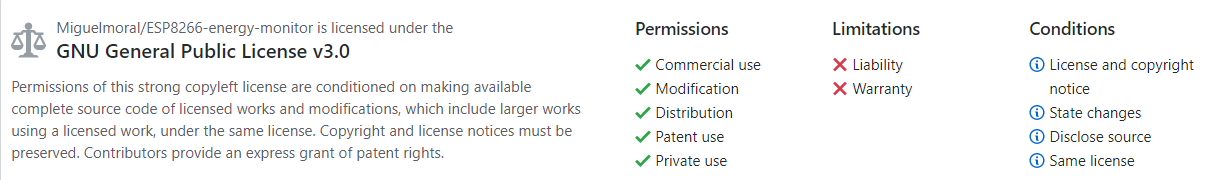
\includegraphics[scale=0.6]{imagenes/gnugpl.png}
	\caption[Resumen de la licencia GNU GPL v3]{Resumen de la licencia GNU GPL v3 Fuente: \cite{gitlicencia} }
	\label{fig:grafGNU}
\end{figure}

Todas las bibliotecas utilizadas para este proyecto tienen una licencia de software libre.

\section{Hardware principal utilizado en el proyecto}

En esta sección se hablará sobre el Hardware principal utilizado para realizar este proyecto.

\subsection{ESP8266}

Para la realización de este proyecto se ha decidido utilizar una Placa ESP8266 frente a otras soluciones más habituales como suele ser Arduino.

Uno de los problemas del Arduino es que carece de conexión a internet. Si necesitamos dotar a nuestro proyecto de conexión WIFI tendremos que utilizar un chip para proporcionar a nuestro Arduino de dicha conexión. Aquí es donde entra en juego el chip ESP8266 creado con la idea de ser utilizado en proyectos de IoT y poder dotar al Arduino de conexión WiFi.

En el mercado existen diferentes fabricantes de placas que integran el chip ESP8266, pero para este proyecto se va a utilizar la placa NodeMCU v2.

En 2014 salta al mercado el kit de desarrollo de código libre NodeMCU. Inicialmente se trataba únicamente de un firmware en lenguaje LUA. Pero dos meses después el proyecto se amplia y desarrollan una placa de hardware libre. Se trata de la primera versión conocida como v0.9 o V1. Estas placas cuentan con una memoria de 4 KBytes y un almacenamiento de 4 MBytes \cite{nodemcuwikipedia}. Existen actualmente tres versiones diferentes de esta placa. Todas estas versiones son muy similares de la primera a la segunda generación tan solo cambia la anchura de la placa ya que con la placa v1 se ocupaban los 10 pines que traen las protoboards de tamaño standard, la v2 soluciona este problema haciendo la placa un poco más estrecha dejando una fila de pines en cada lado de placa cuando colocamos esta en una protoboard, además de substituir el chip ESP12 para pasar a montar el nuevo chip mejorado ESP12E. Al tratarse de hardware libre cualquier compañía interesada puede fabricar las placas, en el caso de estas dos primeras versiones han sido producidas por la empresa Amica, sin embarco la v3 la ha sacado al mercado la empresa Lolin. Esta nueva versión v3 no aporta cambios sustanciales con respecto a la v1 y la v2, tan solo un puerto USB más robusto y ha utilizado uno de los pines reservados para alimentación USB para proporcionar un pin adicional de GND \cite{nodemcuversiones} .

Principalmente las ventajas que nos ofrece esta placa son su bajo precio, su simplicidad tanto a la hora de programar como a la hora de realizar las conexiones, la posibilidad de soportar distintos lenguajes de programación como son (LUA, MicrPhython o Arduino) y sobretodo su conexión WiFi.

En la imagen (\ref{fig:nodemcu}) podemos ver todas las conexiones de las que dispone la versión v2 de la placa NodeMCU.

\begin{figure}[H]
	\centering
	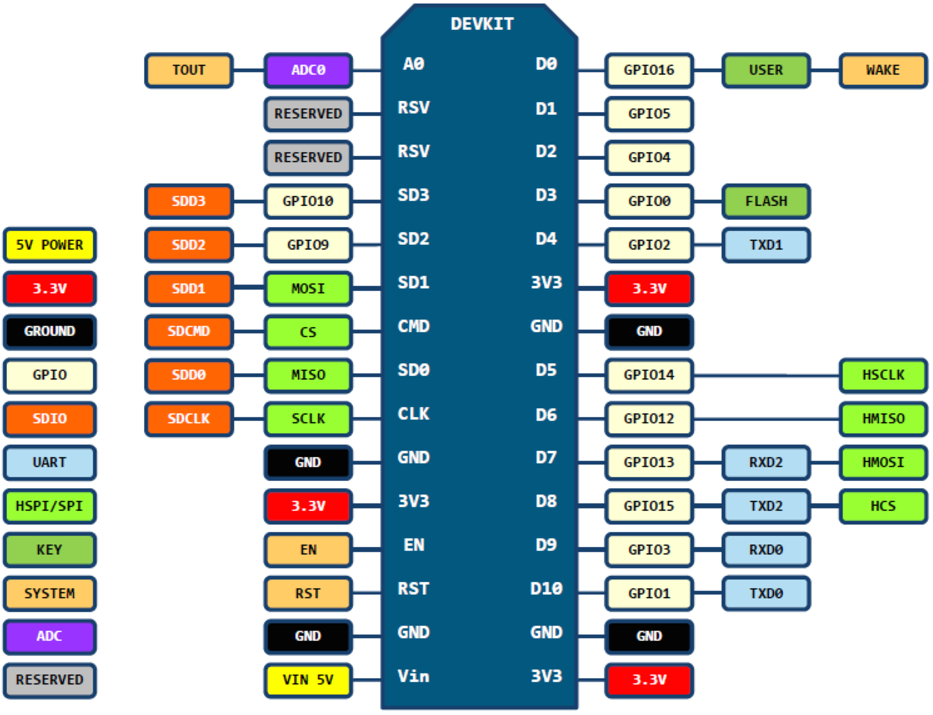
\includegraphics[scale=0.6]{imagenes/nodemcu.png}
	\caption[NodeMCU.]{NodeMCU. Fuente: \cite{nodemcuversiones}}
	\label{fig:nodemcu}
\end{figure}


\subsection{Raspberry Pi}

Se trata de una pequeña placa base que monta un procesador del fabricante Broadcom, en concreto el modelo BCM2835. Se trata de un procesador con arquitectura ARM a 1GHz de velocidad, además cuenta con una GPU VideoCore IV y una memoria de 512 MB, el almacenamiento del dispositivo dependerá la la tarjeta SD que el cliente introduzca en la placa aunque no es muy recomendable introducir SD de gran capacidad ya que las SD soportan un número limitado de lecturas y escrituras, por lo que al estar manejando un sistema operativo estas SD no suelen tener un tiempo de vida muy largo debido a la cantidad de lecturas y escrituras que tienen que realizar. Además con lo que al almacenamiento se refiere la Raspberry soporta tanto discos duros externos como pendrives por lo que el almacenamiento en este dispositivo no es ningún problema \cite{raspberrywikipedia}.

Con respecto al software podemos escoger entre una gran cantidad de sistemas operativos los cuales están disponibles para esta placa. Los más populares están basados en GNU/Linux como pueden ser Raspbian tanto su versión Lite sin entorno gráfico más dedicada al uso como servidor o su versión de escritorio una versión específica para raspberry derivada de Debian. Estos sistemas operativos se pueden descargar completamente gratis de la web oficial \cite{raspbianoficial}. Una vez descargados tan solo tendremos que flashearlos en una tarjeta SD y tendremos el sistema operativo elegido funcionando sin ningún tipo de problema en nuestra raspberry. Existen además otros sistemas operativos para esta placa permitiendo utilizarla no solo como un pequeño ordenador o como un servidor, gracias a sistemas operativos como OpenELEC podremos utilizar este dispositivo como un centro multimedia, incluso existen sistemas operativos para emular videojuegos.

Además de su reducido precio para la gran potencia que nos ofrece, una de las mayores virtudes de esta placa es el gran número de conexiones que nos ofrece. Esta placa cuenta con las siguientes conexiones (modelo Pi 2) : \cite{raspberrywikipedia}

\begin{itemize}
	\item\textbf{Puertos USB: } Dispone de 4 puertos USB 2.0.
	\item\textbf{Salidas de video: } Conector RCA, HDMI e interfaz DSI para conectar un panel LCD.
	\item\textbf{Salidas de audio: } Cuenta con un conector Jack de 3,5mm y una salida HDMI.
	\item\textbf{Conectividad de red: } Dispone de una entrada Ethernet (RJ-45).
	\item\textbf{Alimentación: } Integra una entrada microUSB de 5V para poder alimentar la placa de manera sencilla.
\end{itemize}

En la imagen (\ref{fig:Raspberryimg}) podremos ver todas las conexiones de manera más clara.

\begin{figure}[H]
	\centering
	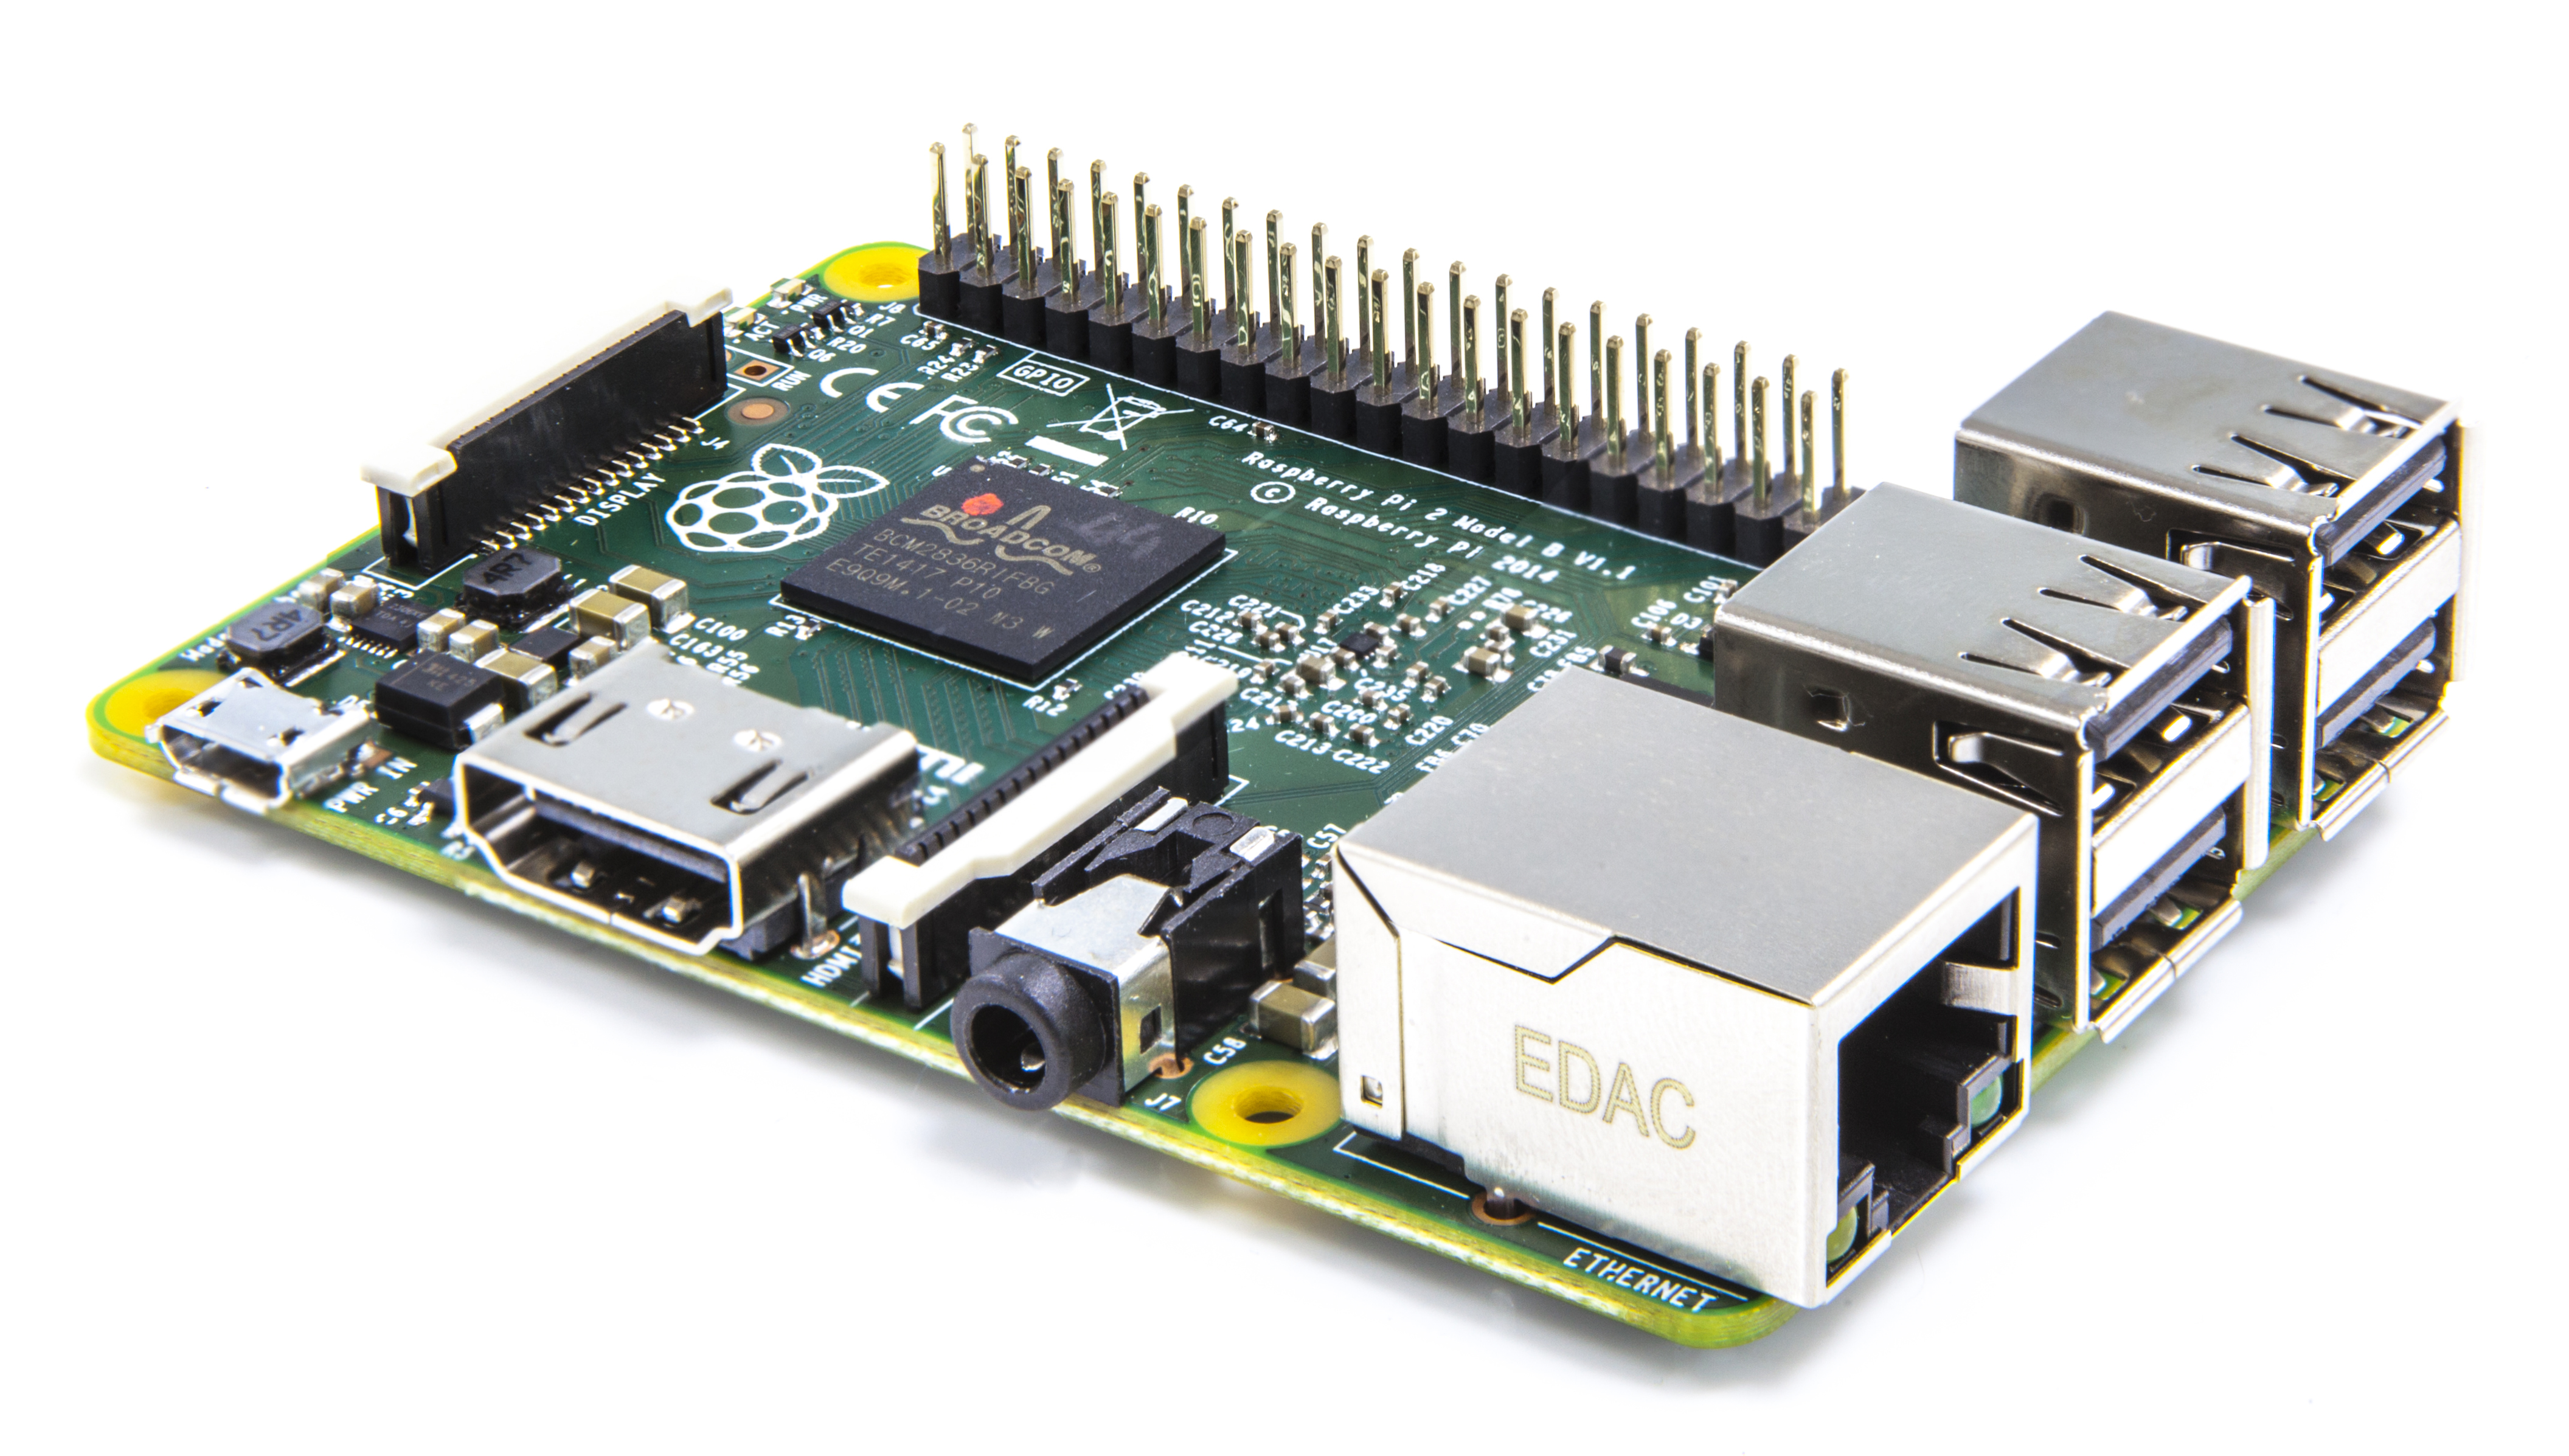
\includegraphics[scale=0.4]{imagenes/raspberry.jpg}
	\caption[Raspberry.]{Raspberry. Fuente: \cite{imagenraspberry}}
	\label{fig:Raspberryimg}
\end{figure}



\section{Sensores de energía en el mercado actual.}
Antes de empezar el proyecto es necesario analizar las soluciones que nos ofrece el mercado actualmente. A continuación vamos a repasar los puntos fuertes y los puntos débiles de estas soluciones.

\begin{itemize}
\item\textbf{Efergy Technologies ENGAGE HUB 1.1: } Se trata de un sensor que se conecta de forma inalámbrica con sus propios servidores donde se almacenará la información que se recoja en nuestro hogar. Pone a disposición del cliente un portal web gratuito que le permitirá consultar los datos recogidos, cuenta además con una aplicación para android y para IOS.Este dispositivo permite conectar una pantalla externa de la propia marca la cuál no está incluida en el precio. A un precio de 112,08 \$ (\EUR{99,9}).\cite{Efergy}
	
\begin{figure}[H]
	\centering
	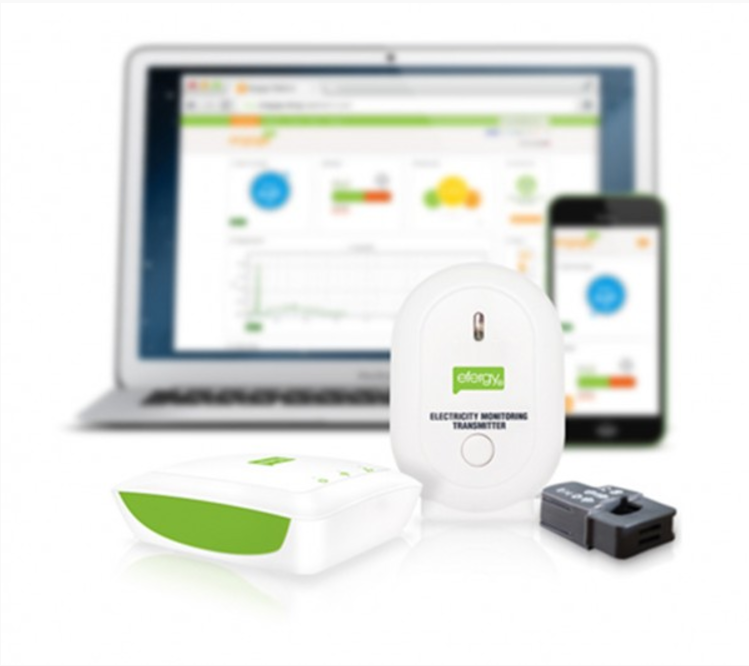
\includegraphics[scale=0.9]{imagenes/efergy.png}
	\caption[Efergy ENGAGE HUB 1.1]{Efergy ENGAGE HUB 1.1. Fuente: \cite{Efergy}}
	\label{fig:Efergy}
\end{figure}


\item\textbf{Neurio W1-HEM Home Energy Monitor: } Ofrece actualización de los datos segundo a segundo. Infraestructura basada en la nube permitiendo acceder a los datos desde cualquier lugar y aplicaciones web y para dispositivos android e IOS. Una de las ventajas de este dispositivo es que cuenta con una API pública que nos permitirá incorporar los datos que recojamos de forma sencilla. Precio en Amazon EEUU 219,99 \$. \cite{Neur}
	
	
\begin{figure}[H]
	\centering
	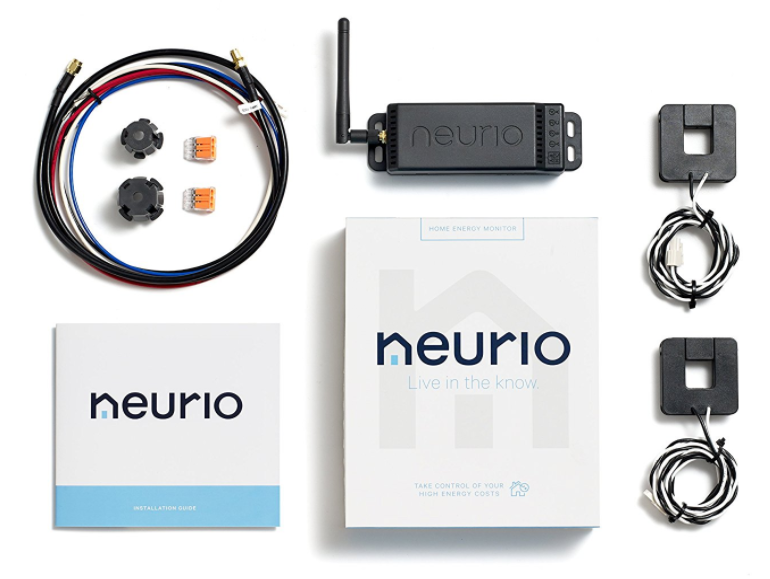
\includegraphics[scale=0.7]{imagenes/neurio.png}
	\caption[Neurio W1-HEM energy monitor]{Neurio W1-HEM energy monitor. Fuente: \cite{Neur}}
	\label{fig:neurio}
\end{figure}

\item\textbf{Efergy Technologies Elite Classic: } Es el modelo más básico de la compañía Efergy. Cuenta con una pequeña pantalla en blanco y negro que permite consultar los datos que recoge del sensor. La información que se recoge del sensor se actualiza cada 10 segundos por defecto pudiendo configurarlo para que se produzca cada 15 o 20 segundos. Este modelo no permite enviar datos a la nube, a no ser que compremos el accesorio engage. Precio de 61,50 \$ (\EUR{54,90}).\cite{Efergyclassic}

\begin{figure}[H]
	\centering
	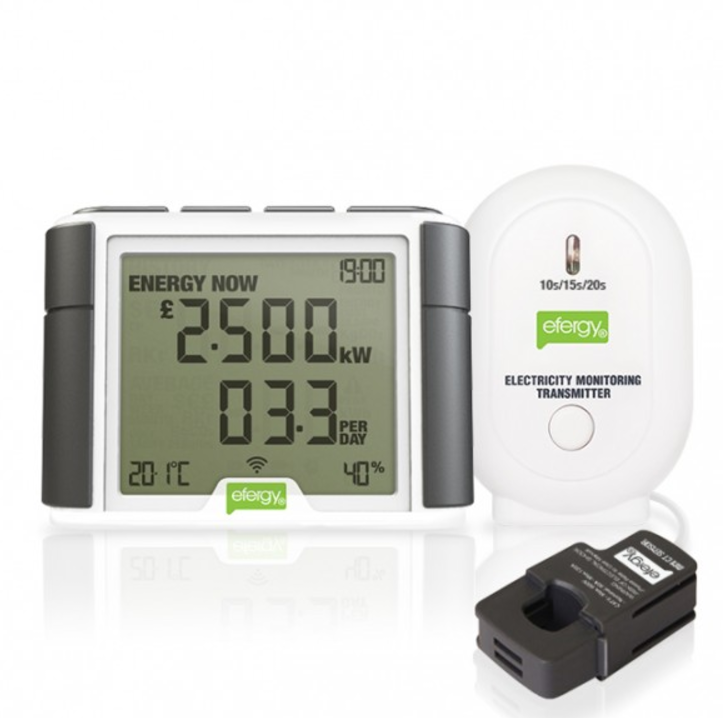
\includegraphics[scale=0.9]{imagenes/efergyclassic.png}
	\caption[Efergy Elite Classic.]{Efergy Elite Classic. Fuente: \cite{Efergyclassic}}
	\label{fig:Efergyclassic}
\end{figure}

\item\textbf{Floureon Power Meter Energy Monitor US TS-836A: } Se trata del modelo más básico de todos los que estamos analizando, siendo además el más económico de todos. Este dispositivo no se puede considerar directamente como IoT ya que tan solo muestra sus datos mediante una pantalla incorporada en el dispositivo, pero no existe la posibilidad de transmitir estos datos. Otro inconveniente de este dispositivo es que no permite monitorizar toda la casa ya que este dispositivo ha de conectarse en un enchufe. Su precio es de 20 \$ (\EUR{17,80}) más envío.\cite{floureon}

\begin{figure}[H]
	\centering
	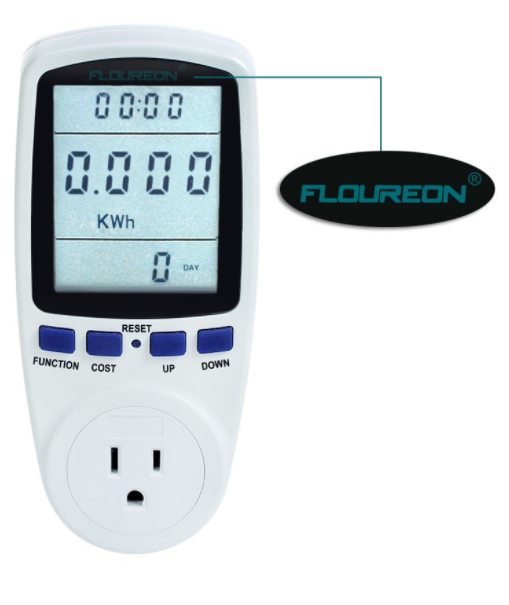
\includegraphics[scale=0.9]{imagenes/floureon.png}
	\caption[Floureon Power Meter Energy Monitor.]{Floureon Power Meter Energy Monitor. Fuente: \cite{floureon}}
	\label{fig:floureon}
\end{figure}

\item\textbf{Belkin Conserve Insight: } Se trata de un dispositivo muy similar al Floureon. La principal diferencia la encontramos en que el dispositivo de la marca Belkin nos muestra además la cantidad de dióxido de carbono que producimos según el consumo eléctrico que esté midiendo el aparato, aunque realmente se trata de una simple multiplicación. Cabe mencionar que algunos usuarios informan que la calidad de este aparato no es buena, llegando algunos usuarios incluso a comentar que el dispositivo se les ha quemado con el consiguiente riesgo de incendio. Al igual que pasaba con el dispositivo de la marca Floureon no se nos ofrece la posibilidad de almacenar los datos que recoge el sensor en ningún servidor ya que el aparato no dispone de conectividad para poder comunicarse con el servidor. El precio de este aparato es de 29,99 \$ (\EUR{26,70}). \cite{Belkin}

\begin{figure}[H]
	\centering
	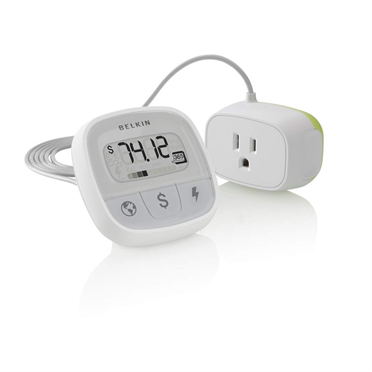
\includegraphics{imagenes/belkin.jpg}
	\caption[Belkin Conserve Insight.]{Belkin Conserve Insight. Fuente: \cite{Belkin}}
	\label{fig:Belkin}
\end{figure}

\item\textbf{EmonTx V3: } La propuesta opensource que nos trae OpenEnergyMonitor nos permitirá conectar un total de 4 sensores de energía no invasivos. Conectividad vía RF 433/868 MHz o posibilidad de dotar al aparato con conectividad WiFi utilizando una placa ESP8266. Incorpora la opción de hacer medidas de temperatura además de hacer una monitorización de energía. Permite enviar los datos recogidos por el sensor mediante RF 433/868 MHz a una raspberry o a cualquier servidor en caso de utilizar la conexión WiFi del ESP8266. A un precio de \EUR{65}.\cite{emonTx}

\begin{figure}[H]
	\centering
	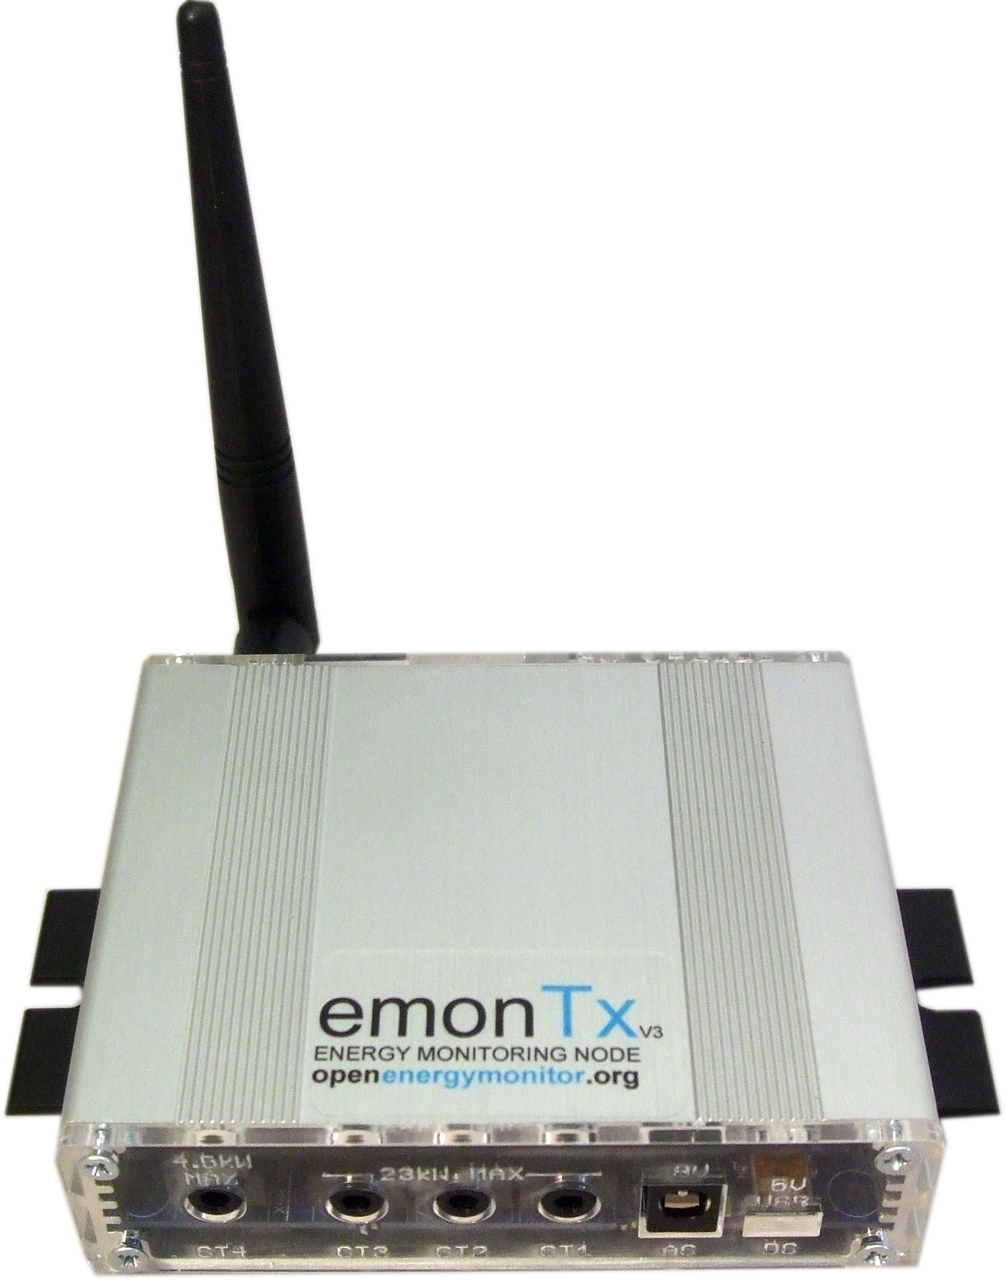
\includegraphics[scale=0.25]{imagenes/emonTx.png}
	\caption[EmonTx V3.]{EmonTx V3. Fuente: \cite{emonTx}}
	\label{fig:emonTx}
\end{figure}

\item\textbf{Sense home energy system: } Este sensor tiene como idea que nuestra casa se comunique con nosotros. De modo que la casa nos dirá durante cuanto tiempo hemos estado viendo la televisión, o durante cuanto tiempo ha estado encendida una bombilla. Este sistema no tiene que aprender nuestros hábitos durante un periodo de tiempo para reconocer que aparato está consumiendo electricidad en cada momento si no que ya conoce el modelo de consumo eléctrico de ciertos electrodomésticos y aparatos eléctricos de la casa. Este aparato se comunica mediante WiFi para mandar la información que recogen sus sensores a un servidor de la propia empresa. Podremos visualizar nuestros consumos y demás datos a través de un portal web o mediante una app disponible para Android e IOS. El precio de este producto ronda los \EUR{265}.\cite{Senseoficial}

\begin{figure}[H]
	\centering
	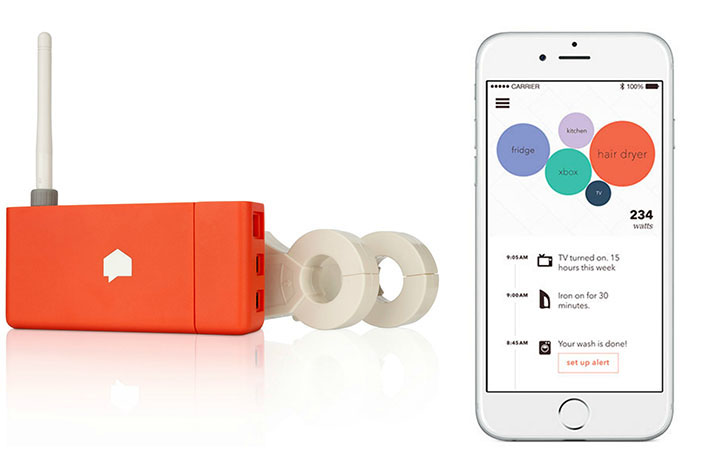
\includegraphics[scale=0.5]{imagenes/sense.jpg}
	\caption[Sense.]{Sense. Fuente: \cite{Senseimagen}}
	\label{fig:emonTx}
\end{figure}

\item\textbf{British Gas energy monitor: } Debido a una iniciativa por parte del gobierno de gran bretaña que busca reducir el consumo eléctrico de los hogares la compañía de luz y gas británica British gas podrán pedir un monitor de energía y gas de forma gratuita incluyendo su instalación. Los datos recogidos por el sensor se mandan monitor utilizando Zigbee y estos datos se mandan directamente vía GPRS a la compañía British Gas haciendo que no se tengan que revisar los consumos de cada casa ya que se actualizan automáticamente. Actualmente este dispositivo tan solo se puede conseguir siendo cliente de la compañía British Gas. \cite{BritishGas}

\begin{figure}[H]
	\centering
	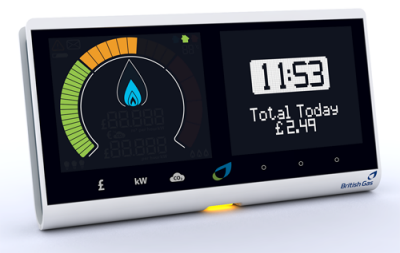
\includegraphics[scale=0.7]{imagenes/britishgas.png}
	\caption[British Gas.]{British Gas. Fuente: \cite{BritishGas}}
	\label{fig:britishgas}
\end{figure}

	
\end{itemize}




\section{Tabla comparativa de sensores de energía en el mercado.}
Mediante la tabla (\ref{tabla:monitores}) se pretende resumir de forma más clara y sencilla toda la información dada en la sección anterior de cada uno de los dispositivos que se nombraron.

\begin{landscape}
	
	\begin{table}
	
			\resizebox{25cm}{!} {
				\begin{tabular}{|l||c|c|c|c|c|c|c|c|c|}
					\hline
					Modelo & Dispone API & Tiempo refresco & Protocolo Comunicación & Monitorización solar & Pantalla para visualizar datos & Cloud & Precio\EUR{} \\
					\hline \hline 
					Efergy Engage & \checkmark & Seleccionable 10, 15 o 20 sec & Wifi & Con accesorio & Con módulo Elite classic & \checkmark & 99.9\\ \hline
					Efergy elite  & \checkmark & Seleccionable 10, 15 o 20 sec & Sin especificar & Con accesorio & \checkmark & Con módulo Engage & 195.86\\ \hline
					Neurio & \checkmark & Instantáneo & Wifi 802.1 b/n/g & Con accesorio & $\times$ & \checkmark & 54.90\\ \hline
					Floureon & $\times$ & Instantáneo & No transmite datos & $\times$ & \checkmark & $\times$ & 17.80\\ \hline
					Belkin & $\times$ & Instantáneo & No transmite datos & $\times$ & \checkmark & $\times$ & 26.70\\ \hline
					EmonTx V3 & $\times$ & Instantáneo & RF 433/868 MHz & $\times$ & \checkmark & \checkmark & 65\\ \hline
					Sense & $\times$ & Instantáneo & Wifi, Bluetooth & Con accesorio & $\times$ & \checkmark & 265\\ \hline
					British Gas & $\times$ & Instantáneo & GPRS, Zigbee & $\times$ & \checkmark & \checkmark & -\\ \hline
				\end{tabular}
			}
			\caption{Monitores de energía en el mercado.}
			\label{tabla:monitores}
	\end{table}

\end{landscape}

Teniendo en cuenta las diferencias entre modelos y los precios de cada aparato existen dos alternativas principales en función de la necesidad del cliente las mejores opciones serían :

\begin{itemize}
	\item\textbf{Monitorizar el consumo de un solo electrodoméstico: } En caso de que el cliente necesite un dispositivo sencillo al menor precio posible, recomendaría el dispositivo de la marca Belkin  (Conserve Insight). Si lo comparamos frente a su competidor el Floureon la diferencia de precio es de tan solo unos 9 euros permitiéndonos el dispositivo de la marca Belkin visualizar la cantidad de dióxido de carbono que producimos. Por lo demás ambos dispositivos son muy similares.
	\item\textbf{Monitorizar el consumo de toda la casa: } Como podemos observar en el caso de querer monitorizar la casa entera el precio de los dispositivos se dispara. En mi opinión el mejor dispositivo de los que se han presentado es el Efergy Technologies Elite Classic, además de ser el más económico de los tres modelos que permiten monitorizar el consumo de toda la casa podremos actualizar el dispositivo y comprar el módulo Engage para almacenar nuestros datos en los servidores que nos brinda la empresa Efergy y poder visualizar nuestros consumos desde su plataforma web o sus aplicaciones para dispositivos móviles. No considero que sea rentable pagar la diferencia de precio existente con el modelo que nos ofrece la compañia Neurio ya que no existen diferencias que justifiquen este sobreprecio. Sin embargo la característica que nos trae Sense que nos permite comunicarnos con nuestra casa viendo consumos exclusivos de cada aparato me parece muy interesante aunque en mi opinión no justifica el alto precio del producto.El EmonTx no me parece mala opción pero es necesario documentarse un poco para poder empezar a utilizarlo si no se tiene experiencia.
	
\end{itemize}

\section{Porqué hacer nuestro propio monitor}

Como podemos observar en el mercado existen diversas propuestas que se pueden adaptar a las necesidades que buscamos cubrir, pero en este proyecto se va a llevar a cabo el diseño y construcción de un monitor con características similares a los que existen. Algunos de los motivos que nos han llevado a realizar nuestro propio monitor son los siguientes:

\begin{itemize}
	\item\textbf{Aprender: } Durante todo el proceso se van a adquirir conocimientos en diversas áreas como pueden ser hardware, electrónica, etc.
	\item\textbf{Precios: } Podremos además comprobar si el precio de realizar nuestro propio dispositivo es razonable con respecto a los precios que nos ofrecen aparatos comerciales.
	\item\textbf{No usar servicios externos: } A la hora de enviar los datos recogidos con nuestro dispositivo tendremos total libertad de escoger en que servidor se van a almacenar estos, pudiendo ser tanto un servidor local como cualquier otro servidor.
\end{itemize}

%
\chapter{Objetivos}

En este proyecto el objetivo principal \textbf{OBJ-G} es desarrollar un dispositivo libre que permita monitorizar el consumo eléctrico tanto del hogar como de un dispositivo específico y que permita transmitir estos datos de forma inalámbrica, todo ello al menor precio posible.
Podemos dividir este objetivo principal en los siguientes objetivos principales:

\begin{itemize}
	\item\textbf{OBJ-P1} Diseño hardware con una placa que permita la conexión inalambrica WiFi para poder enviar los datos recogidos de un sensor no invasivo.
	
	\item\textbf{OBJ-P2} Implementación del firmware que permite capturar los datos que recoge el sensor y enviar estos datos vía WiFi.
	
	\item\textbf{OBJ-P3} Creación de un servidor web para poder almacenar los datos recibidos en una base de datos y que permitirá al usuario revisar consumos.
	
	\item\textbf{OBJ-P4} Documentación de todo el proyecto.
	
	
\end{itemize}

Una vez tenemos todos los objetivos principales definidos vamos a dividirlos en objetivos más específicos. Dentro de estos subobjetivos existirán algunos de ellos obligatorios para que la funcionalidad del proyecto sea completa y otros opcionales que servirán para perfeccionar el proyecto, pero estos no serán vitales para su correcto funcionamiento:

\begin{itemize}
	\item\textbf{OBJ-P1-OB1} Investigación de sensores de corriente no invasivos existentes en el mercado y como conectarlos a distintas placas.
	
	\item\textbf{OBJ-P1-OB2} Investigación para seleccionar la placa que mejor se adapte a este proyecto que cuente con conexión WiFi.
		
	
	\item\textbf{OBJ-P1-OB3} Montaje del primer prototipo con los componentes seleccionados anteriormente.
	
	\item\textbf{OBJ-P1-OP1} Mejora de este primer prototipo para añadir funcionalidades al proyecto.
	
	\item\textbf{OBJ-P1-OP2} Realizar todo el montaje de los componentes en un PCB para que el dispositivo tenga un buen acabado.
	
	\item\textbf{OBJ-P2-OB1} Decidir en que lenguaje programar la placa escogida y que IDE utilizar.
	
	\item\textbf{OBJ-P2-OB2} Implementar un primer firmware para asegurar que el hardware funciona adecuadamente.
	
	\item\textbf{OBJ-P2-OB3} Decidir en que formato y como se van a enviar las mediciones recogidas por la placa al servidor.
	
	\item\textbf{OBJ-P2-OP1} Mejorar el firmware para enviar más parámetros al servidor.
	
	\item\textbf{OBJ-P3-OB1} Selección de framework para crear la aplicación web.
	
	\item\textbf{OBJ-P3-OB2} Seleccionar el sistema de base de datos que vamos a utilizar para almacenar los datos recibidos por la placa.
	
	\item\textbf{OBJ-P3-OB3} Decidir donde alojar la base de datos y la aplicación web.
	
	\item\textbf{OBJ-P3-OB4} Implementar la aplicación web.
	
	\item\textbf{OBJ-P3-OP1} Mejorar la aplicación web para mostrar más información al usuario.
	
	\item\textbf{OBJ-P4-OB1} Subir a un repositorio de GitHub todo lo necesario para que las personas que estén interesadas puedan utilizar este proyecto por su cuenta de manera sencilla.
	
	\item\textbf{OBJ-P4-OB1} Realizar toda la documentación del proyecto en Latex siguiendo la plantilla ofrecida por la UGR.
	
	\item\textbf{OBJ-P4-OP1} Hacer un estudio de los consumos de algún electrodoméstico.
	
\end{itemize}

\section{Diagrama objetivos}

\begin{landscape}

	\begin{figure}
		\centering
		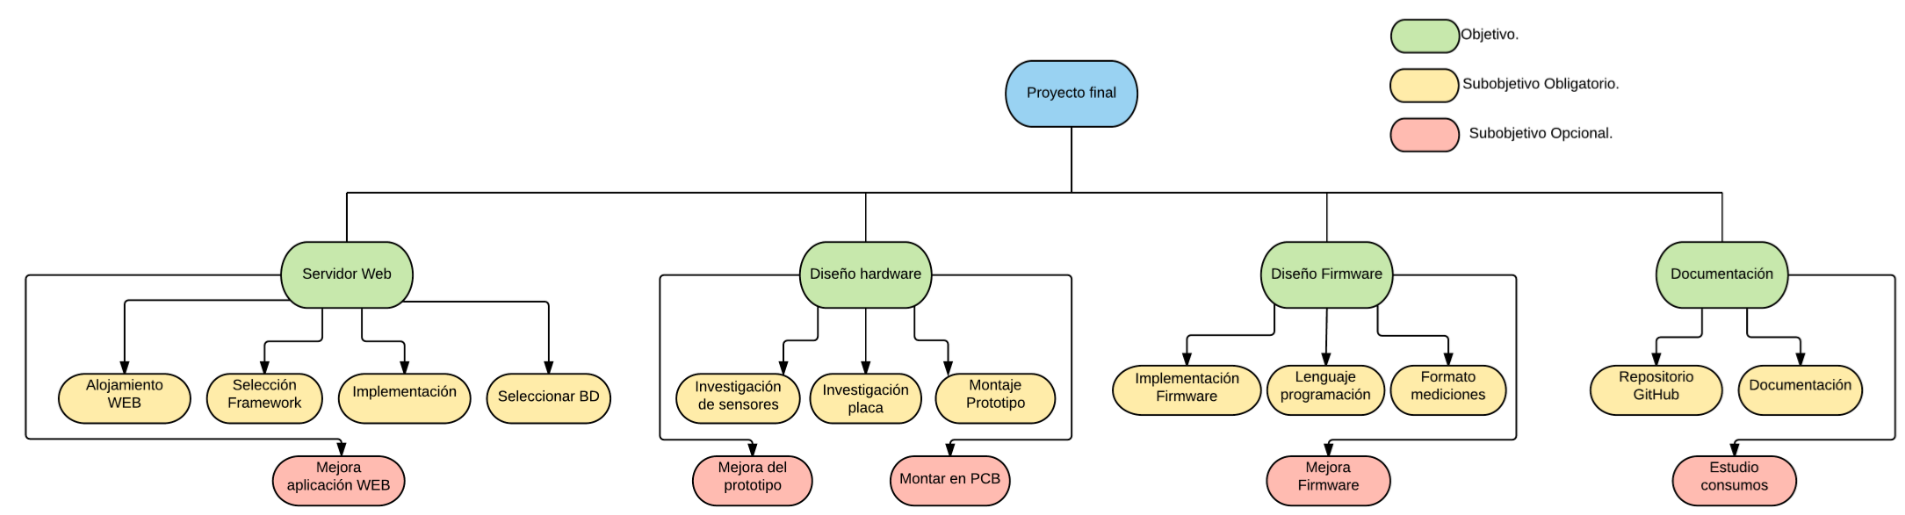
\includegraphics[scale=0.5]{imagenes/diagramaObjetivos.png}
		\caption{Diagrama de objetivos}
		\label{fig:Diagrama de objetivos}
	\end{figure}
	
\end{landscape}

\section{Conocimientos necesarios para alcanzar estos objetivos.}

Algunos de estos conocimientos han sido adquiridos tras cursar las asignaturas que se indicarán a continuación y otros de los conocimientos han sido adquiridos por mi propia cuenta al tener que realizar algunos de los objetivos de este proyecto:

\begin{itemize}
	\item\textbf{Conocimientos adquiridos mediante asignaturas de la carrera:}
	\begin{itemize}
		\item\textbf{Desarrollo de aplicaciones para internet:} Los conocimientos adquiridos tras cursar esta asignatura me han servido para poder realizar la web utilizando flask, además de conocer el lenguaje de programación python y las bases de datos NoSQL como MongoDB.
		\item\textbf{Infraestructura virtual:} Se han puesto en uso los conocimientos a la hora de utilizar git y GitHub.
		\item\textbf{Fundamentos de software:} Entre el temario de esta asignatura se encuentra una parte dedicada a la realización de scripts y algunos comandos básico de Linux que se han puesto en práctica para la realización de este proyecto.
		\item\textbf{Fundamentos de programación:} Donde se ven conceptos básicos sobre programación en c++ que en cierto modo han servido como base para realizar toda la parte de programación tanto web como a la hora de programar la placa.
	\end{itemize}
	\item\textbf{Conocimientos adquiridos gracias a la realización de este proyecto:}
		\begin{itemize}
		\item\textbf{\LaTeX:} He tenido que aprender Latex para poder realizar toda la documentación de este proyecto.
		\item\textbf{Arduino IDE:} A la hora de programar la placa he tenido que aprender como usar este IDE.
		\item\textbf{Electrónica básica:} Para poder llevar a cabo el montaje de todos los circuitos.
		\item\textbf{Raspberry Pi:} He necesitado adquirir conocimientos básicos para poder montar un servidor en una RaspberryPi.
		\item\textbf{Soldadura:} Conocimientos básicos de soldadura que nos permiten soldar pistas de estaño en la PCB para poder materializar los prototipos presentados en la protoboard en una placa real. 
		\item\textbf{Electricidad:} Necesario conocer un mínimo para poder calcular el Irms y la potencia ya que no tenia ningún tipo de conocimiento en este campo antes de realizar el proyecto.
	\end{itemize}
\end{itemize}




%
\chapter{Planificación y presupuesto}

La metodología de trabajo utilizada a la hora de desarrollar este proyecto está basada en la creación y prueba de prototipos de manera iterativa, ya que al tratarse de un proyecto de desarrollo de hardware principalmente se ha considerado que esta es la mejor manera de comprobar si el prototipo funciona como se esperaba o existe algún tipo de fallo el cuál puede ser arreglado en el siguiente prototipo. Además dados los escasos conocimientos iniciales que se tenían en electrónica y electricidad este esquema de desarrollo ha permitido aprender de manera más gradual y práctica. Esta metodología de trabajo se verá reflejada en la planificación propuesta inicialmente que se especificará a continuación así como una estimación del coste total del proyecto.

\section{Planificación del trabajo}
Esta planificación fue realizada cuando aún no se había empezado a trabajar en el proyecto por lo tanto algunos de estos plazos finalmente no se han cumplido tal y como se esperaba.

\begin{itemize}
	\item\textbf{Módulo hardware:}
		\begin{itemize}
			\item Reunión con la persona interesada en el proyecto 16/02/2017 - 16/02/2017. 
			\item Investigación de todas las alternativas existentes para llevar a cabo esta parte del proyecto 16/02/2017- 22/02/2017.
			\item Adquirir todos los componentes necesarios para esta parte comparando los precios y el producto en si que ofrecía cada tienda 22/02/2017 - 23/02/2017.
			\item Diseño de prototipos 23/02/2017 - 17/03/2017.
			\item Montaje de los prototipos diseñados con realización de pruebas para comprobar su correcto funcionamiento 1/03/2017 - 14/04/2017.
			\item Diseño de las placas de las versiones finales 14/04/2017 - 21/04/2017.
			\item Soldar las versiones finales en una PCB 21/04/2017 - 28/04/2017.
			\item Probar las versiones finales 28/04/2017 - 03/05/2017.
			\item Diseño de cajas donde irá colocada la pcb y el resto de componentes de la versión final 03/05/2017 - 04/05/2017.
			\item Montaje de las cajas 04/05/2017 - 05/05/2017.
		\end{itemize}
	\item\textbf{Módulo firmware:}
		\begin{itemize}
			\item Reunión con la persona interesada en el proyecto 16/02/2107 - 16/02/2017. 
			\item Investigación de todas las alternativas existentes para llevar a cabo esta parte del proyecto 16/02/2017- 22/02/2017.
			\item Desarrollo de toda la parte firmware que se subirá a la placa ESP8266 1/03/2017 - 02/06/2017.
			\item Pruebas 02/06/2017 - 09/06/2017.
		\end{itemize}
		\item\textbf{Parte servidor:}
	\begin{itemize}
		\item Reunión con la persona interesada en el proyecto 09/06/2017 - 09/06/2017. 
		\item Investigación de todas las alternativas existentes para llevar a cabo esta parte del proyecto 09/06/2017 - 16/06/2017.
		\item Realización de una aplicación web para el proyecto 16/06/2017 - 30/06/2017.
		\item Alojar dicha aplicación web en un servidor (RaspberryPi) 19/06/2017 - 06/07/2017.
		\item Pruebas 01/07/2017 - 10/07/2017.
	\end{itemize}
\end{itemize}

\begin{landscape}
	
	\begin{figure}
		\centering
		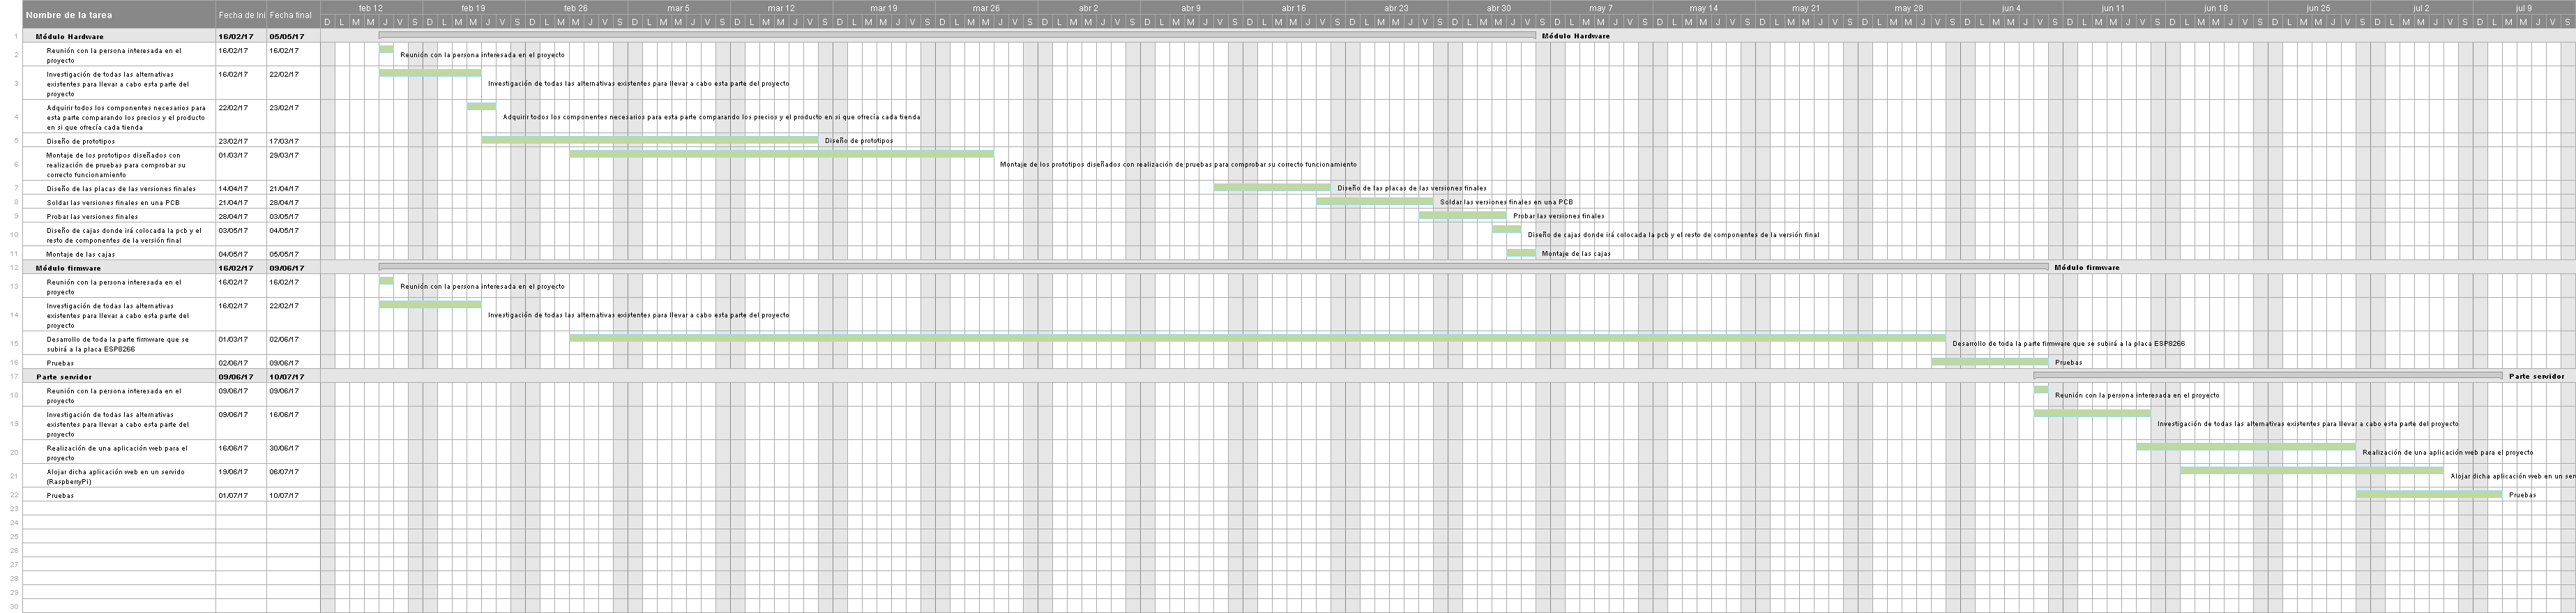
\includegraphics[scale=0.15]{imagenes/gantt.png}
		\caption{Diagrama de Gantt}
		\label{fig:Diagrama de Gantt}
	\end{figure}
	
\end{landscape}

\section{Presupuesto del proyecto}

A continuación se especificará un presupuesto con los costes del proyecto:

\begin{itemize}
	\item\textbf{Hardware y componentes electrónicos :} En el apartado número 4 se especifica detalladamente el coste de todo el hardware adquirido el cuál se sitúa en los \textbf{\EUR{40.47}}, a este tenemos que sumarle otros \EUR{36.76} ya que algunos de los componentes se compraron más de una vez ya que resultaron dañados mientras se realizaron las pruebas. Obteniendo por lo tanto un coste final de \textbf{\EUR{77.23}}
	
	\item\textbf{Parte servidor :} En esta parte el único coste ha sido la adquisición de una Raspberry Pi ya que el sistema operativo utilizado para la Raspberry tiene una licencia gratuita.Las herramientas de desarrollo utilizadas para esta parte son gratuitas como el editor de textos Atom \cite{atom}. El precio de la Raspberry está en torno a los \textbf{\EUR{39.90}}.
	
	\item\textbf{Parte firmware :} Para el desarrollo de esta parte se ha utilizado únicamente software libre en concreto Arduino IDE \cite{arduinoide}, además de bibliotecas con licencia de software libre, por lo tanto el coste ha sido \textbf{\EUR{0}}.
	
	\item\textbf{Horas de trabajo:} El proyecto en total ha tenido una duración total de 7 meses. Para contar las horas de trabajo vamos a suponer que los fines de semana no se ha trabajado por lo tanto si se cuentan los días laborables desde el 16/02/2017 hasta el 2/09/2017 obtenemos un total de 137 días laborables. Trabajando durante una media de 2 horas diarias para poder compatibilizar estudios y la realización de este proyecto obtenemos un total de 274 horas dedicadas a este proyecto. Suponiendo que cada hora se cobre a \EUR{12.5} obtenemos un total de \textbf{\EUR{3425}}.
	
	\item\textbf{Coste del ordenador utilizado para el desarrollo de este proyecto :} Para calcular este coste calcularemos la depreciación \cite{depreciacion} de este producto partiendo de que el precio base son \EUR{800}, calculamos que el ordenador tendrá aproximadamente una vida útil de 5 años con un valor residual de \EUR{100}. Calculamos la base de amortización $ Base amortizacion = valor inicial - valor residual $    por lo que nos queda un valor residual de \EUR{700}. Dividimos este valor entre la vida útil estimada para este ordenador y nos queda un total de \EUR{140} al año. Durante los 7 meses que ha durado este proyecto hemos supuesto que el tiempo que el ordenador ha estado siendo usado son unos 2 meses, por lo tanto obtenemos un precio de \textbf{\EUR{23.33}}.
	
	\item\textbf{Total :} Sumando todos los costes tenemos un total de \textbf{\EUR{3565.46}}
	
\end{itemize}
%
\chapter{Módulo hardware}
La idea principal de este proyecto es utilizar todo el hardware libre posible, que entre otras ventajas nos permite abaratar los costes que es una de las ideas principales del proyecto.

En este capítulo se describirá detalladamente todo el hardware que se ha utilizado para llevar a cabo este proyecto.

\section{Requisitos}

A continuación se recogerán los requisitos tanto funcionales como no funcionales del módulo hardware:

\subsection{Requisitos funcionales}

\begin{itemize}
	\item\textbf{RF1: } Recoger las mediciones mediante un sensor.
	\item\textbf{RF2: } Manejar la información obtenida para mostrar información util para el usuario.
	\item\textbf{RF3: } Enviar dicha información a un servidor para poder tener todos los datos almacenados.
	\item\textbf{RF4 (Opcional): } Mostrar dicha información al usuario mediante una pantalla.
\end{itemize}

\subsection{Requisitos no funcionales}

\begin{itemize}
	\item\textbf{RNF1: } La placa que se diseñe debe tener unas dimensiones reducidad para reducir costes entre otras cosas.
	\item\textbf{RNF2: } Las dimensiones de la caja donde se alojará la placa tendrá las dimensiones lo más reducidas posible.
	\item\textbf{RNF3: } El aparato debe permitir su instalación sin necesidad de contar con la ayuda de un electricista o de modificar cualquier elemento de la instalación eléctrica donde queramos medir los consumos.
\end{itemize}

\section{Planificación}

\begin{itemize}
	\item\textbf{Fase 1: } Reunión con la persona interesada para concretar los detalles del proyecto que se quieren llevar a cabo.
	\begin{itemize}
		\item\textbf{Recopilar la información}  sobre los detalles que nos especifique la persona interesada.
		\item\textbf{Estudiar}  si es factible llevar a cabo las peticiones que se nos han hecho.
		\item Tener una \textbf{segunda reunión} para concretar las cosas que se pueden llevar a cabo y las que no.
	\end{itemize}
	\item\textbf{Fase 2: } Estudio de las tecnologías disponibles y compra del material.
	\begin{itemize}
		\item\textbf{Revisar}  que componentes de hardware libre se adecuan para llevar a cabo nuestro proyecto
		\item\textbf{Estudiar}  cuales de esos componentes son los más adecuados basándonos en aspectos como el precio, la comunidad o la disponibilidad que tengan estos componentes.
		\item\textbf{Comparar} los distintos precios que nos ofrecen las tiendas para la compra de estos componentes y buscar la que nos ofrezca la mejor relación entre un tiempo de envío no demasiado alto y un precio adecuado.
	\end{itemize}
	\item\textbf{Fase 3: } Diseño y montaje.
	\begin{itemize}
		\item\textbf{Diseño}  de los esquemas de montaje.
		\item\textbf{Montaje}  de dichos esquemas utilizando una protoboard\cite{protoboard}.
		\item\textbf{Montaje y pruebas} con distintos prototipos.
		\item\textbf{Soldar} la PCB con los componentes correspondientes.
		\item\textbf{Fabricación} de distintas carcasas para alojar la placa final
	\end{itemize}
	\item\textbf{Fase 4: } Pruebas.
	\begin{itemize}
		\item\textbf{Pruebas}  de los distintos prototipos para comprobar su correcto funcionamiento.
	\end{itemize}
	
\end{itemize}


\section{Arquitectura del sistema}

En este apartado se van a detallar los componentes que se han utilizado para desarrollar cada uno de los módulos hardware que componen este sistema.

\subsection{Módulo principal}
Podríamos haber optado por el uso de otra placa como puede ser un Arduino \cite{arduino}. El principal inconveniente que presenta esta placa para su utilización en este proyecto es que carece de conexión inalámbrica WiFi por lo tanto para poder mandar los datos al servidor vía WiFi se necesitaría un módulo a parte para dotar al Arduino de conexión WiFi.

Para permitir que el Arduino disponga de conexión WiFi se utiliza el módulo WiFi ESP8266. En el caso de este proyecto unicamente la placa NodeMCU Amica cubre todas nuestras necesidades las cuales son:

\begin{itemize}
	\item Conexión inalámbrica WiFi.
	\item Conexión I2C.
	\item Bajo coste.
	\item Tamaño de la placa muy reducido.
\end{itemize}

De esta manera conseguimos a parte de hacer un diseño más sencillo abaratar costes, ya que no será necesario adquirir además un Arduino.

Las especificaciones del ESP8266 se pueden consultar en el apartado 1.1.1.

\subsection{Módulo sensor}
En este proyecto es necesaria la utilización de un sensor de corriente no invasivo para permitir una fácil instalación del dispositivo sin necesidad de modificar ningún cable de la instalación eléctrica.

Existen en el mercado distintos sensores de energía no invasivos como el que nos ofrece la marca SparkFun \cite{sparkfun}.

Para este proyecto vamos a utilizar el sensor de la marca YHDC ya que es el que más versiones nos ofrece y la disponibilidad del mismo es mayor que el de otros sensores de similares características.

En concreto se va a usar la versión de 100A que nos permitirá medir cargas de hasta 100A.

En esta imagen (\ref{fig:pinza}) podemos ver que la salida del sensor se produce a través de un jack de audio por el canal de la izquierda y el sleeve. En las demás versiones de pinzas de la marca con la de 30A contamos con una resistencia de carga que hace que la salida sea una señal de voltaje. Sin embargo en el caso de la pinza de 100A como podemos ver en el esquema (\ref{fig:pinza}) en la figura de la izquierda la señal de salida que nos proporciona es continua ya que carece de una resistencia de carga por lo tanto tendremos que añadir a nuestro esquema eléctrico una resistencia de carga para convertir a una señal de voltaje.  

\begin{figure}[H]
	\centering
	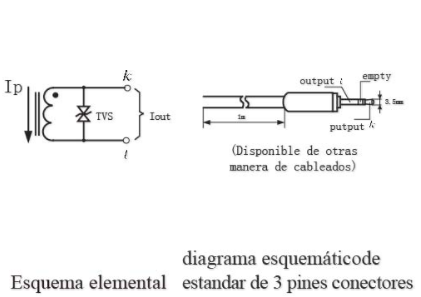
\includegraphics[scale=1]{imagenes/esquemapinza.png}
	\caption[YHDC.]{YHDC. Fuente: \cite{sensorcorriente}}
	\label{fig:pinza}
\end{figure}

\subsection{Módulo conversor analógico digital}
El propio ESP8266 pueda realizar una conversión de una señal analógica a una digital mediante el PIN A0 con una resolución de 10 bits.

Sin embargo si utilizamos el conversor analógico digital ADS 1115 conseguiremos una resolución de 16 bits. Además utilizando la biblioteca Adafruit\textunderscore ADS1015 \cite{adafruitbib} en concreto la función \textit{readADC\textunderscore Differential\textunderscore 0\textunderscore 1()} la cuál nos permite conocer la diferencia de voltaje entre el pin 0 y el pin 1 del ADS esto hace posible que no sea necesario el uso de dos resistencias en paralelo "bias resistor" . Para llevar a cabo nuestro esquema eléctrico tendremos que hacer uso de los pines VDD y GND los cuales alimentaremos a 3,3 V, los pines SCL y SDA para conectarlo al ESP8266 haciendo uso de la conexión I2C y los pines A0 y A1.

Las ventajas que nos ofrece este conversor analógico digital son:

\begin{itemize}
	\item Nos permite tener más precisión.
	\item Conexión I2C con la placa ESP8266.
	\item Elimina la necesidad de incorporar al circuito dos resistencias adicionales.
\end{itemize}


\begin{figure}[H]
	\centering
	\includegraphics[scale=0.6]{imagenes/ads1115.png}
	\caption[ADS1115.]{ADS1115. Fuente: \cite{adsfoto}}
	\label{fig:ads}
\end{figure}
\subsection{Módulo pantalla}

Como se especificó en el capítulo 2 de objetivos, el módulo de la pantalla corresponde a un objetivo opcional que finalmente se ha decidido incluir en el proyecto final.

A parte de ver la información detallada sobre los consumos en la web puede ser interesante para el usuario disponer de la información de forma inmediata y cómoda mediante una pantalla integrada en el propio dispositivo.

Debido a su bajo precio y que muchas de las soluciones para la medición de consumos eléctricos existentes en el mercado como se vio en el apartado 1.2 disponen se decidió que sería una buena idea incluirla en el diseño. Si la persona que desee realizar este proyecto no ve necesaria la utilización de esta pantalla se podría quitar sin ningún tipo de problema teniendo de esta manera la misma versión del dispositivo con las mismas funcionalidades pero sin la pantalla. 

Se trata de una pantalla LCD de 16x02 adquirida con un adaptador I2C directamente soldado a los pines que facilita de esta forma la conexión con el ESP8266. Gracias a la conexión I2C podemos conectar sin ningún tipo de problema a los puertos D1 y D2 de nuestro ESP8266 (puertos por defecto para la comunicación I2C en el ESP8266) especificando con que puerto queremos comunicarnos no tendremos ningún tipo de problema a la hora de que tanto el conversor de señal analógico digital (ADS1115) y el LCD compartan la conexión con los puertos D1 y D2.

\begin{figure}[H]
	\centering
	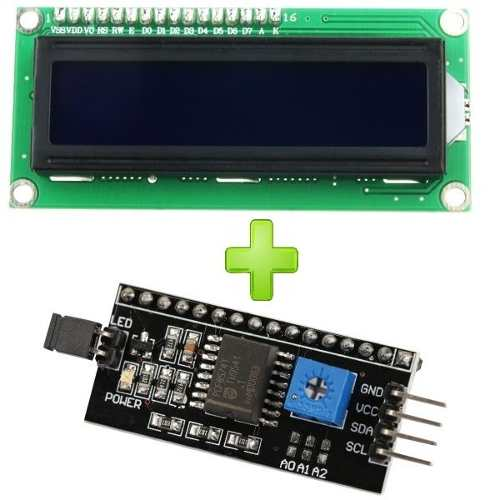
\includegraphics[scale=0.5]{imagenes/lcdi2c.jpg}
	\caption{LCD 16x02 y módulo I2C}
	\label{fig:lcdi2c}
\end{figure}

\section{Coste unitario}
Los precios mostrados a continuación (\ref{tabla:precios}) pueden variar en función de la tienda donde se adquieran los productos además pueden variar su precio a la alza o a la baja con el paso del tiempo. No están reflejados los gastos de envío de los productos ya que varían mucho en función de la web donde se adquieran.

Cabe destacar que los precios de algunos de los productos que aparecen en la tabla como puede ser la PCB están calculados restando el precio de la parte utilizada para llevar a cabo el proyecto al precio de la PCB completa.


\begin{table}[H]
	\begin{center}
		\begin{tabular}{|l|l|}
			\hline
			Producto & Precio \\
			\hline \hline
			NodeMcu ESP8266 CP2102 & \EUR{5.54} \\ \hline
			YHDC Non-Invasive AC Current Sensor [100A/30A] & \EUR{5.41} \\ \hline
			ADS1115 16bits ADC+PGA  & \EUR{2.45} \\ \hline
			Pantalla LCD 16x02 (Opcional)  & \EUR{3.49} \\ \hline
			40x cable macho macho  & \EUR{1.80} \\ \hline
			Estaño  & \EUR{0.40} \\ \hline
			Tira pines macho  & \EUR{1} \\ \hline
			Tira pines hembra  & \EUR{3} \\ \hline
			Trozo de placa experimental prototipo (PCB) & \EUR{2} \\ \hline
			Resistencias, jack hembra, conector entrada alimentación & \EUR{4} \\ \hline
			Tornillos, tuercas & \EUR{0.50} \\ \hline
			\textbf{Total} & \textbf{\EUR{29.59}} \\ \hline
			\textbf{Total sin Pantalla LCD } & \textbf{\EUR{26.10}} \\ \hline
		\end{tabular}
		\caption{Listado de precios.}
		\label{tabla:precios}
	\end{center}
\end{table}

\section{Prototipos}

Todos los diseños de estos prototipos se han realizado con el programa Fritzing antes de llevar a cabo pruebas en la protoboard. Todos estos prototipos se han montado en una protoboard para ahorrarnos de esta forma tener que soldar y gastar más material cada vez que se quisiera probar un nuevo diseño.

En este apartado se detallan las mejoras y fallos de cada uno de los 4 diseños que se analizaron para la construcción de este proyecto:

\begin{itemize}
	\item \textbf{Prototipo 1: } Se trata de la versión inicial con la que comenzó este proyecto. Es un diseño básico que no cuenta ni con pantalla para mostrar información instantánea de los datos que está recogiendo el sensor en cada momento ni con una entrada para poder alimentarlo mediante un conector jack hembra de alimentación. La alimentación de este prototipo iba a través del micro-usb que incorpora la placa NodeMCU. 
	
	\begin{figure}[H]
		\centering
		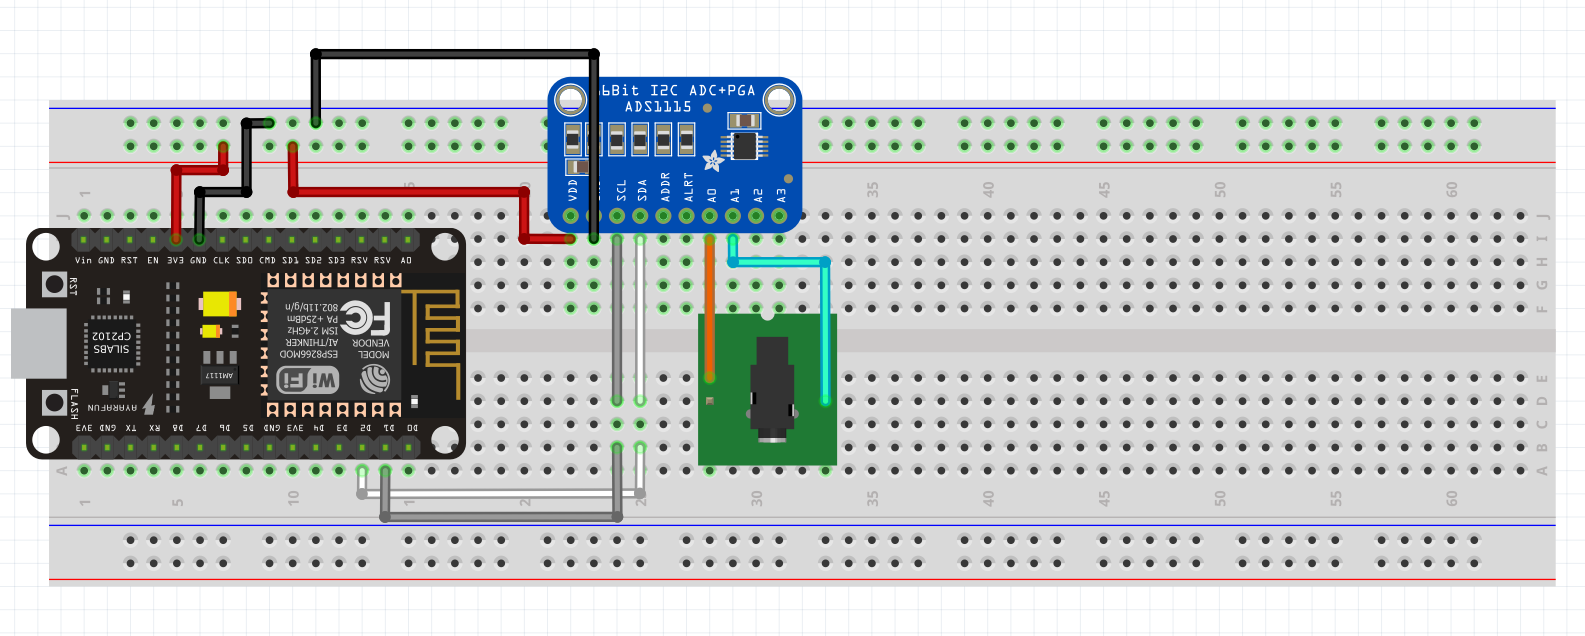
\includegraphics[scale=0.4]{imagenes/protoboardv1.png}
		\caption{Esquema v1}
		\label{fig:protoboardv1}
	\end{figure}

	\item \textbf{Prototipo 2: } Este prototipo incorpora un jack hembra de alimentación que permite alimentar el prototipo ya sea mediante el micro-usb propio de la placa o mediante un cargador de los que suelen usarse normalmente para alimentar otras placas como Arduino con una salida de 5V, lo que se pretendía con este prototipo era usar un único cargador con una salida de 5V para evitar que el usuario cogiera cualquier otro cargador de móvil o de algún otro dispositivo que disponga de una conexión micro usb ya que estos tienen una salida muy diferente los unos de los otros dependiendo de cuál sea el modelo de cargador y la empresa que fabrica el mismo.
	
	\begin{figure}[H]
		\centering
		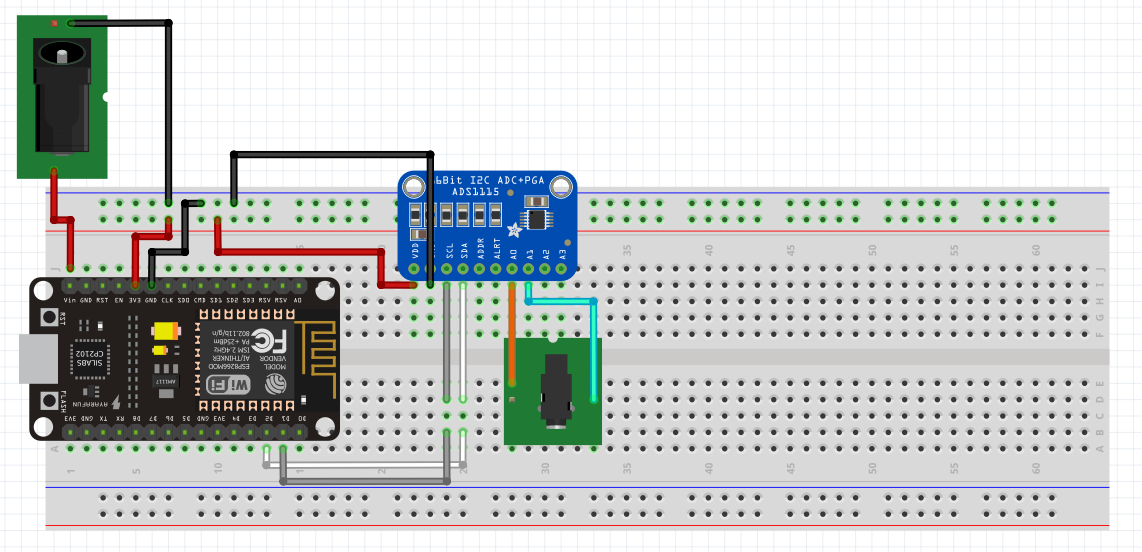
\includegraphics[scale=0.5]{imagenes/protoboardv2.png}
		\caption{Esquema v2}
		\label{fig:protoboardv2}
	\end{figure}
	
	
	\item \textbf{Prototipo 3: } En este diseño se incorpora el amplificador LM358 \cite{lm358} que intenta solucionar los malos resultados de los prototipos vistos anteriormente, pero realmente la solución a estos problemas se encontraban en la forma de poner el sensor de corriente ya que si el sensor rodea los dos cables la lectura no será correcta esta será cercana al 0 ya que los cables tienen corrientes opuestas, estas lecturas cercanas al 0 son el motivo principal por el que se intentó utilizar un amplificador de señal como solución al problema.
	
	\begin{figure}[H]
		\centering
		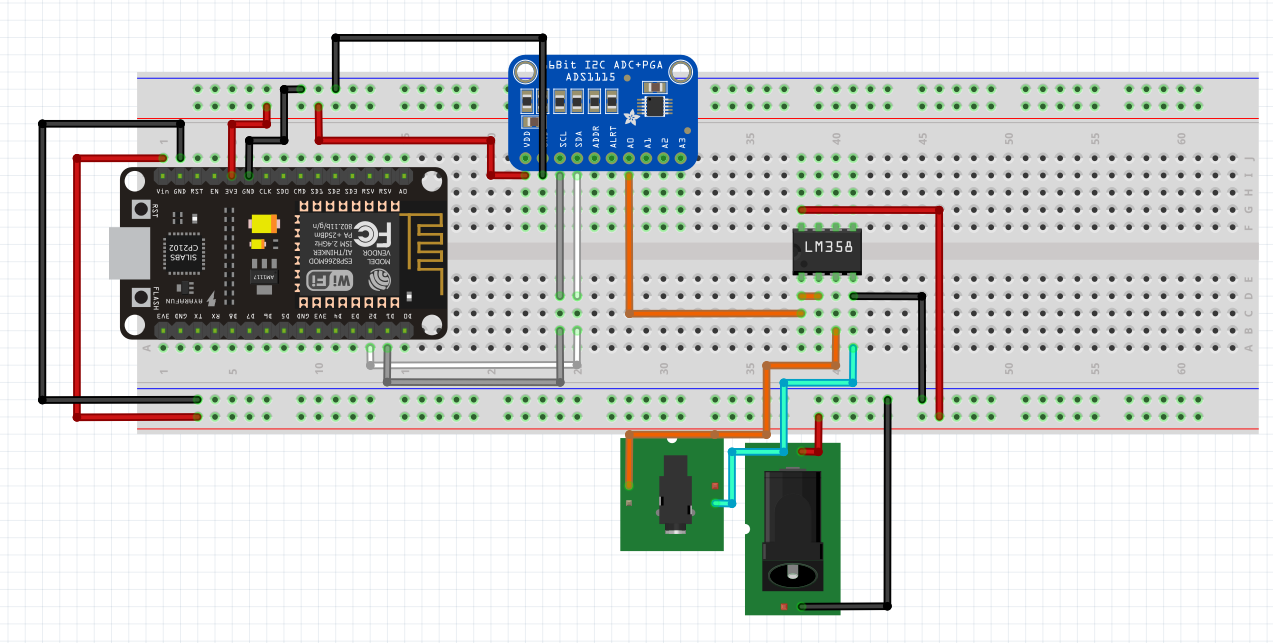
\includegraphics[scale=0.5]{imagenes/protoboardv3.png}
		\caption{Esquema v3}
		\label{fig:protoboardv3}
	\end{figure}
	
	\item \textbf{Prototipo 4: } Se trata de la versión final del proyecto la cuál incluye una pantalla LCD conectada mediante I2C que permite al usuario ver de una manera cómoda la información que está recogiendo en ese momento el sensor.
	
	\begin{figure}[H]
		\centering
		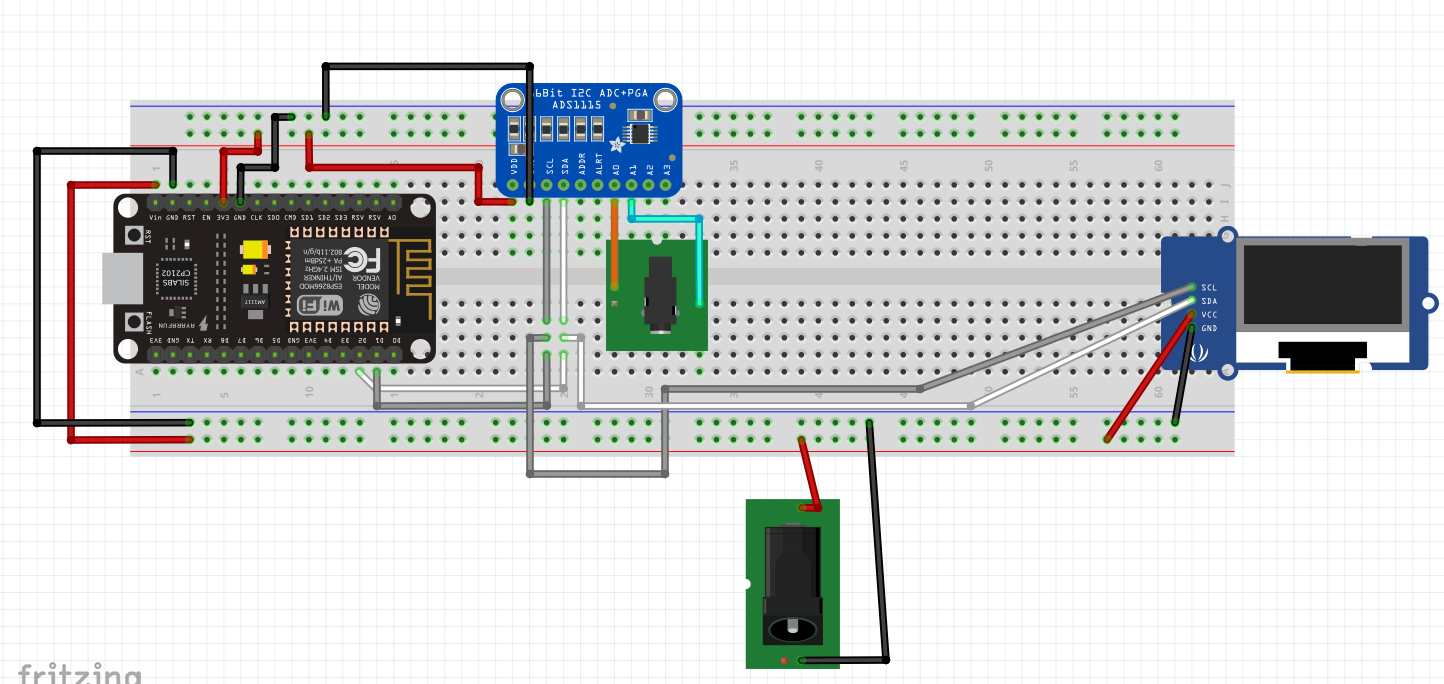
\includegraphics[scale=0.5]{imagenes/protoboardv4.png}
		\caption{Esquema v4}
		\label{fig:protoboardv4}
	\end{figure}
	
\end{itemize}

\section{Versiones finales}

En este apartado se verán los diseños de las dos versiones finales soldando pines hembra a una PCB para facilitar de esta forma el fácil reemplazo de los componentes en caso de que alguno de estos se estropeara o simplemente se quisiera retirar para darle otro uso sin que sufra ningún desperfecto a la hora de retirarlo.

El diseño para soldar las pistas de estaño en la PCB se ha realizado mediante el programa fritzing para asegurar que ninguna de estas pistas se toquen entre ellas provocando de esta forma un mal funcionamiento y al mismo tiempo nos aseguramos de que el tamaño de la placa esta utilizado de la mejor forma posible haciendo la placa lo más pequeña posible por si en un futuro se decidiera producir una gran cantidad de estas placas ahorrar costes de producción además de conseguir un dispositivo de menor tamaño.

\begin{itemize}
	\item \textbf{Versión 1 :} una vez que la persona interesada dio el visto bueno a este diseño (\ref{fig:pcbv1disenio}) realizado soldando pines hembra a una PCB para facilitar el cambio de componentes se pasa a realizar el primer modelo final soldado a una pcb como podemos ver en la imagen (\ref{fig:pcbv1}), observamos 8 conectores hembra donde van colocados los pines correspondientes a la alimentación y comunicación I2C de la pantalla LCD, los conectores para el jack del sensor de corriente y los conectores para conectar el jack de alimentación encargado de dar corriente al ESP8266.

	\begin{figure}[H]
		\centering
		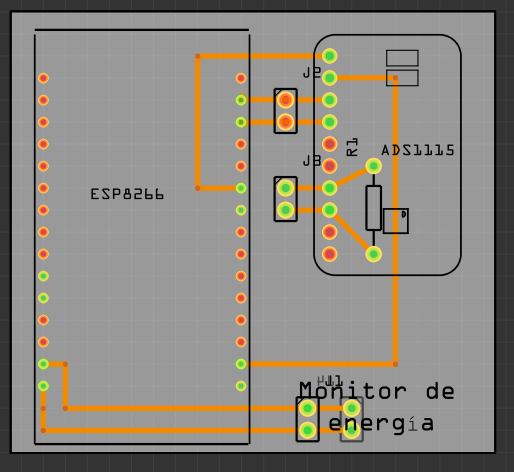
\includegraphics[scale=0.65]{imagenes/v1pcb.png}
		\caption{Esquema PCB versión 1}
		\label{fig:pcbv1disenio}
	\end{figure}

	\begin{figure}[H]
		\centering
		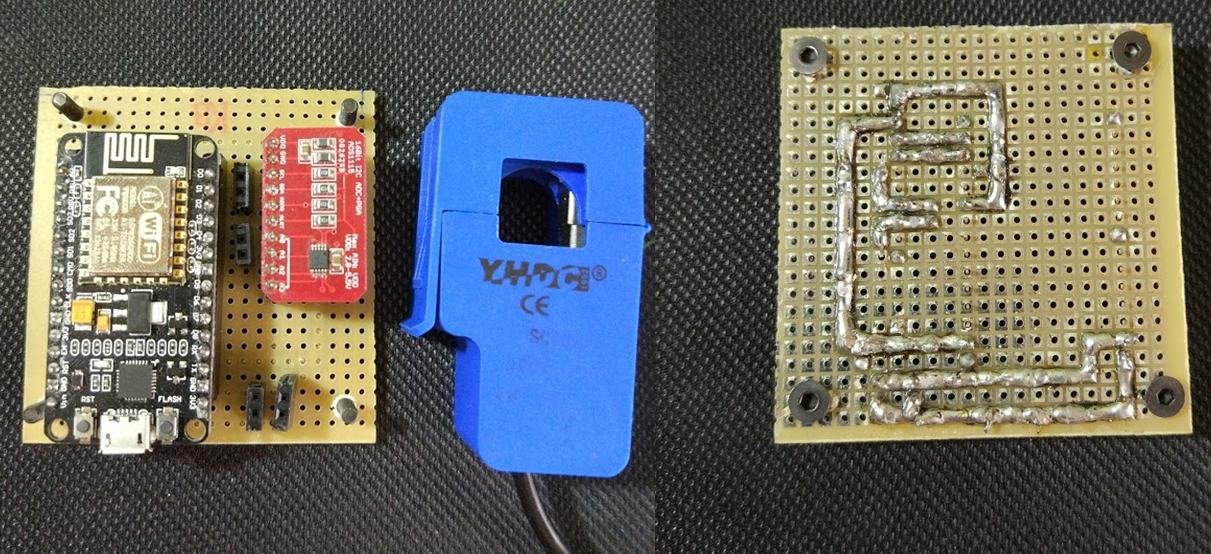
\includegraphics[scale=0.6]{imagenes/pcbv1.png}
		\caption{PCB soldada versión 1}
		\label{fig:pcbv1}
	\end{figure}

	\item \textbf{Versión 2 :} Con la idea de ahorrar espacio y hacer una caja de dimensiones algo más reducidas se estudió un nuevo diseño que permitiera tener uno de los lados de la placa con más espacio, con la idea de hacer la placa más larga que es algo poco importante ya que la caja de todas formas ha de tener el largo suficiente para poder alojar la pantalla LCD, pero un poco más estrecha pudiendo de esta manera colocar la pantalla LCD en uno de los laterales de la caja. Consiguiendo de esta forma que la tapa de la caja pese menos al no tener que soportar el peso de la pantalla LCD.
	
	\begin{figure}[H]
		\centering
		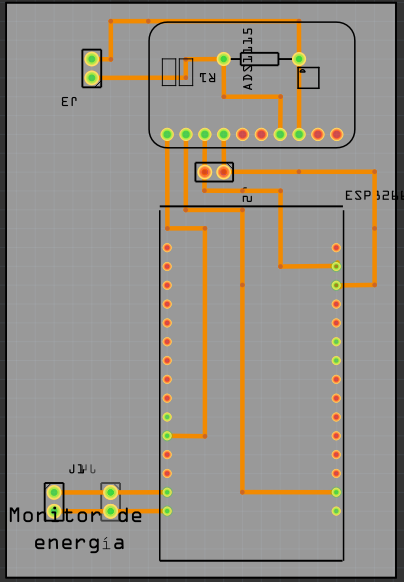
\includegraphics[scale=0.65]{imagenes/diseniopcbv2.png}
		\caption{Esquema PCB versión 2}
		\label{fig:pcbv2disenio}
	\end{figure}
	
	\begin{figure}[H]
		\centering
		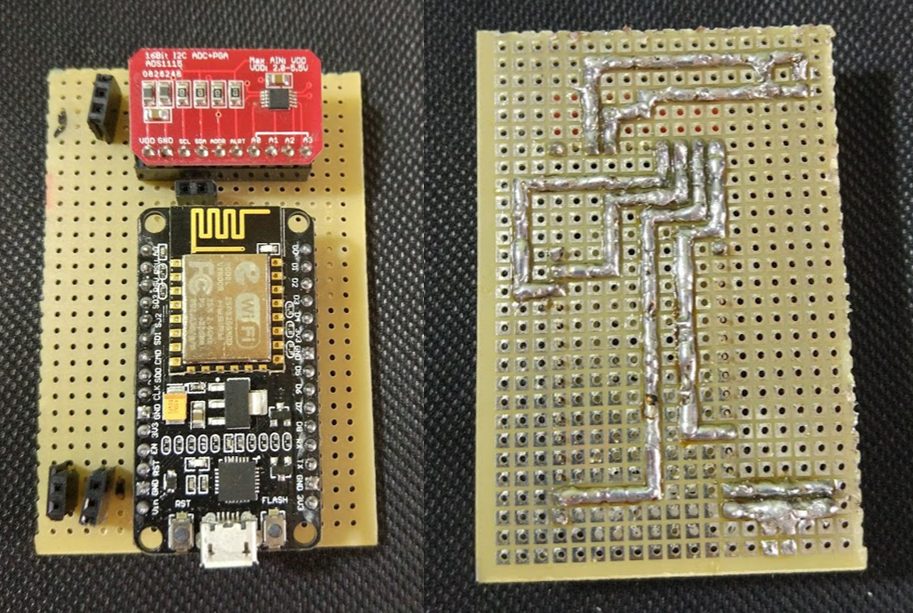
\includegraphics[scale=0.6]{imagenes/pcbv2.png}
		\caption{PCB soldada versión 2}
		\label{fig:pcbv2}
	\end{figure}

\end{itemize}



\section{Montaje de la caja}

Se ha utilizado una cortadora láser para construir las piezas necesarias para alojar la placa y los componentes necesarios en una caja.

Los primeros diseños de la caja están elaborados con DM ya que debido al bajo precio de este material nos permite realizar todas las pruebas que queramos y en caso de que alguna pieza no encaje o el resultado final no sea el esperado siempre podremos repetir esta pieza sin necesidad de desperdiciar un material de precio superior.

\begin{itemize}
	\item \textbf{Versión 1 :} En esta primera versión contamos con una caja básica que permite tener acceso tanto a la entrada micro usb de la placa ESP8266 por si fuera necesario cambiar el firmware de la misma, además de tener acceso a la entrada de jack del sensor de corriente y la entrada para la alimentación tal y como se puede apreciar en la imagen (\ref{fig:cajav1})
	
	\begin{figure}[H]
		\centering
		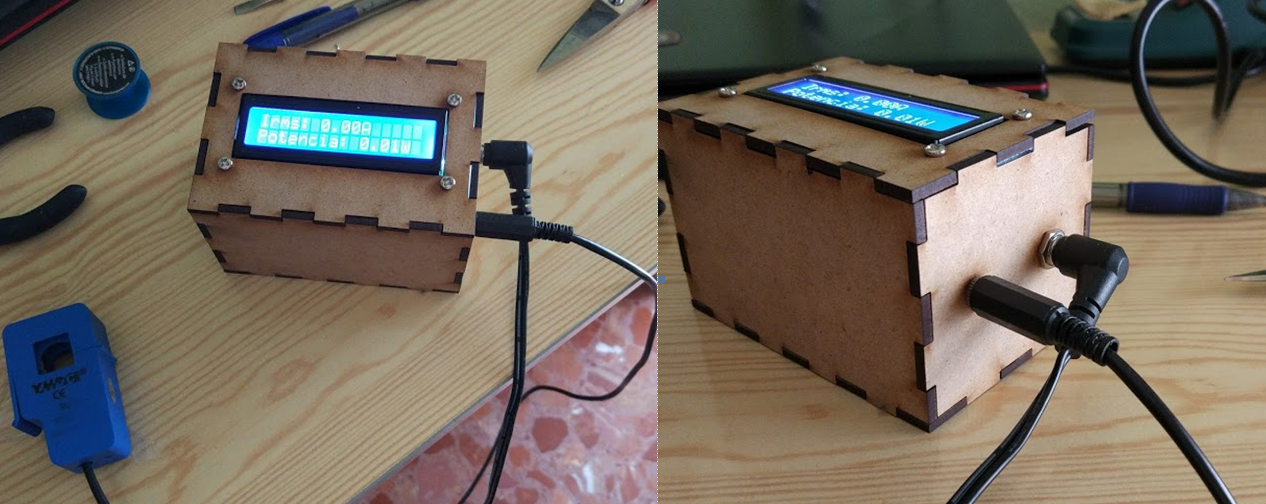
\includegraphics[scale=0.6]{imagenes/cajav1.png}
		\caption{Caja versión 1}
		\label{fig:cajav1}
	\end{figure}
	
	
	\item \textbf{Versión 2 :} En esta segunda versión se mejora la accesibilidad a los componentes que se encuentran en el interior de la caja introduciendo dos pestañas que actúan como bisagras (visibles en la imagen \ref{fig:cajav2}) sujetando la tapa de arriba de la caja la cuál incluye la pantalla haciendo posible de esta forma la apertura de la caja para cambiar cualquier elemento.
	
	\begin{figure}[H]
		\centering
		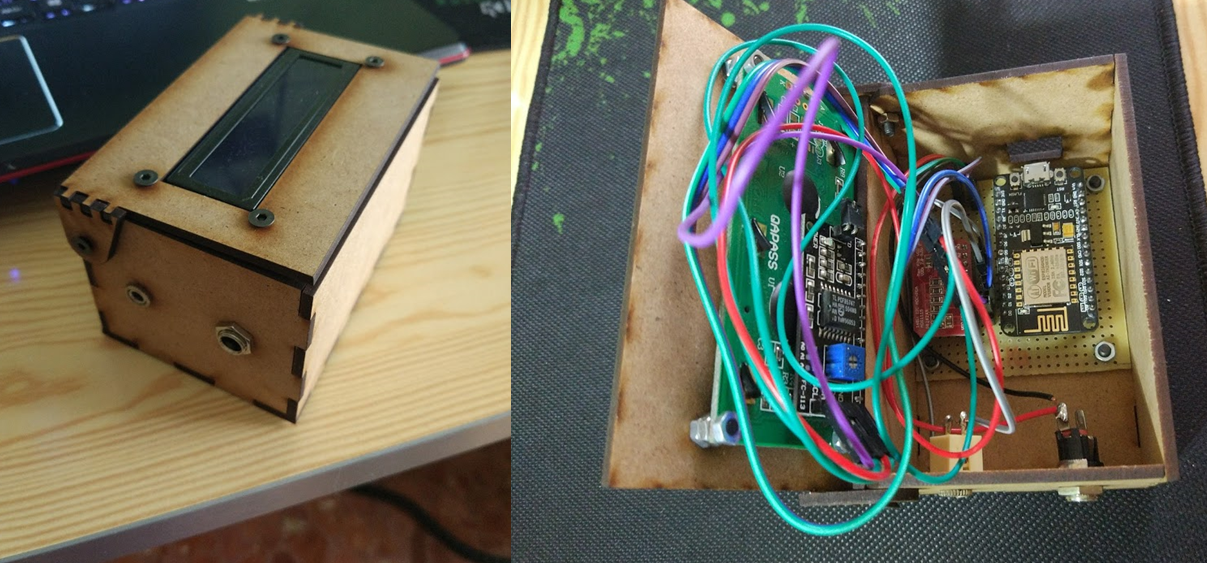
\includegraphics[scale=0.6]{imagenes/cajav2.png}
		\caption{Caja versión 2}
		\label{fig:cajav2}
	\end{figure}
	
\end{itemize}
%
\chapter{Módulo firmware}

En este capítulo se especificarán todos los detalles relacionados con la programación que se ha llevado a cabo en la placa Node MCU ESP8266 \cite{nodemcuwikipedia}.

Esta placa permite al usuario que se programe tanto en LUA \cite{luawikipedia}, MicroPython \cite{micropython} o Arduino \cite{arduino}.

Para la realización de este proyecto se ha elegido el lenguaje de programación de Arduino ya que está basado en C y me siento más cómodo con este lenguaje en comparación con micropython. Además los códigos en C son algo más rápidos y podrían ocupar algo menos de memoria.

\section{Requisitos}

\subsection{Requisitos funcionales}

\begin{itemize}
	\item\textbf{RF1: } Introducir manualmente las credenciales de la conexión WiFi así como el tiempo que tardará en enviarse la información al servidor.
	\item\textbf{RF2: } Comprobar que el dispositivo está correctamente conectado a la red WiFi.
	\item\textbf{RF3: } Recoger la información de los sensores.
	\item\textbf{RF4: } Manejar la información obtenida para mostrar información util para el usuario.
	\item\textbf{RF5: } Mostrar dicha información al usuario mediante una pantalla.
	\item\textbf{RF6: } Enviar dicha información a un servidor para poder tener todos los datos almacenados.
\end{itemize}

\subsection{Requisitos no funcionales}

\begin{itemize}
	\item\textbf{RNF1: } La conexión WiFi del dispositivo ha de ser estable ya que si no los datos no podrían sen enviados al servidor.
	\item\textbf{RNF2: } La información que se muestra en la pantalla LCD se borrará antes de mostrar información nueva para evitar que la información se muestre en lugares de la pantalla inadecuados.
\end{itemize}

\section{Planificación}

\begin{itemize}
	\item\textbf{Fase 1: } Reunión con la persona interesada para concretar los detalles del proyecto que se quieren llevar a cabo.
	\begin{itemize}
		\item\textbf{Recopilar la información}  sobre los detalles que nos especifique la persona interesada.
		\item\textbf{Estudiar}  si es factible llevar a cabo las peticiones que se nos han hecho.
		\item Tener una \textbf{segunda reunión} para concretar las cosas que se pueden llevar a cabo y las que no.
	\end{itemize}
	\item\textbf{Fase 2: } Estudio para decidir en que lenguaje se va a llevar a cabo la programación y como se va proceder para enviar los datos al servidor.
	\begin{itemize}
		\item\textbf{Investigar}  que lenguaje de programación de los 3 (LUA, Micropython, Arduino) que permite el ESP8266 nos interesa más para llevar a cabo este proyecto.
		\item\textbf{Estudiar}  como interpretar los datos recogidos por el sensor para transformarlos en datos legibles por parte del usuario.
		\item\textbf{Estudiar}  cual es la mejor forma de mostrar la información en la pantalla LCD para mostrarla al usuario.
		\item\textbf{Estudiar}  cuál es la mejor forma de mandar los datos al servidor.
		\item\textbf{Estudiar}  cuales son las bibliotecas necesarias para realizar las labores citadas anteriormente.
	\end{itemize}
	\item\textbf{Fase 3: } Programación de los distintos módulos.
	\begin{itemize}
		\item\textbf{Programación}  del módulo de cálculo de irms (valor eficaz) \cite{valoreficaz}.
		\item\textbf{Programación}  del módulo para mostrar la información en la pantalla LCD.
		\item\textbf{Programación} del módulo para enviar la información al servidor.
	\end{itemize}
	\item\textbf{Fase 4: } Pruebas.
	\begin{itemize}
		\item\textbf{Pruebas}  de los distintos módulos que se han programado.
	\end{itemize}
	
\end{itemize}

\section{Arquitectura del firmware}

En este apartado se va a detallar el desarrollo de los distintos módulos que han sido necesarios para la elaboración de este proyecto.

\subsection{Módulo de lectura de sensor y cálculo de irms y potencia}

\begin{itemize}
\item\textbf{Lectura del sensor:}  La lectura de los valores del sensor se realizarán mediante el conversor analógico digital ADS1115. Para ello haremos uso de la biblioteca proporcionada por Adafruit en concreto la Adafruit\textunderscore ADS1x15 \cite{adafruitbib} válida tanto para ls versión 1015 de 12 bits como para la versión 1115 de 16 bits.

Esta biblioteca nos permite leer los valores de los pines desde el A0 hasta el A3 bien sea de forma única \textit{singleended} como calculando la diferencia entre dos pines \textit{differential} a parte de una tercera forma \textit{comparator}. En nuestro caso utilizaremos el modo que calcula la diferencia entre dos pines, es decir la función :

\begin{listing}[style=consola, numbers=none]
	int16_t readADC_Differential_0_1();
\end{listing} 

Esta biblioteca la podemos encontrar en el repositorio de GitHub de Adafruit \cite{adafruitbib}.

\item\textbf{Cálculo de irms y potencia:} Para este proyecto se van a calcular el irms o valor eficaz \cite{valoreficaz} y a partir de ahí la potencia real.

Tras ver los resultados obtenidos por el sensor tal cuál los leemos gracias a la función de la biblioteca de Adafruit mencionada anteriormente. Estamos midiendo corriente alterna, la cuál está cambiando constantemente, por lo tanto tendremos valores con una polaridad negativa y otros con polaridad positiva. Dependiendo del tipo de onda obtenida la fómula que hay que aplicar para calcular el irms cambiará. En la gráfica (\ref{fig:graficasensorraw}) podemos ver que los valores que capta el sensor son tanto positivos como negativos obteniendo esta onda. Por lo tanto no nos interesa obtener ni la media de todos estos valores obtenidos por el sensor ni el valor pico de la onda lo que nos interesa calcular es el valor eficaz. En nuestro caso particular según la bibliografía \cite{mediacuadraticawiki} para calcular el irms de una onda sinosoidal generada al medir corriente alterna la solución es simplemente calcular la media cuadrática aplicando la fórmula de esta media \cite{mediacuadraticawiki} $ \sqrt{\frac{x^2_{1} + x^2_{1} + ... + x^2_{n}}{N}}$.


\begin{figure}[H]
	\centering
	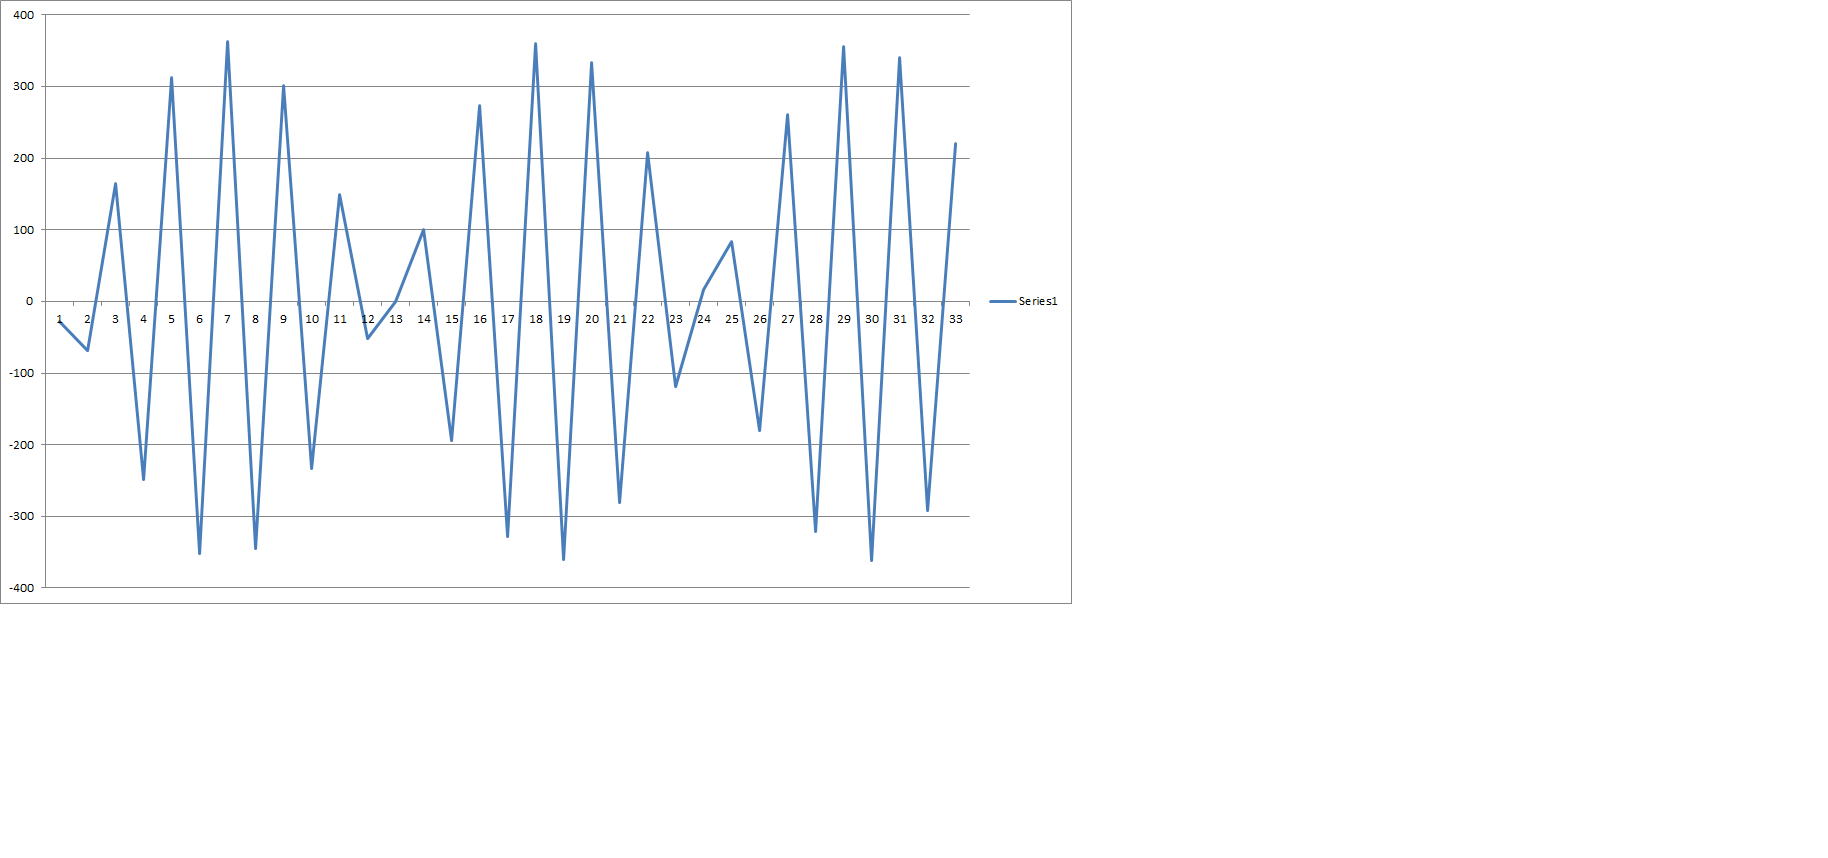
\includegraphics[scale=0.5]{imagenes/datossensorraw.png}
	\caption{Representación datos obtenidos del sensor.}
	\label{fig:graficasensorraw}
\end{figure}

Pero antes de realizar este cálculo tendremos que calcular el offset mediante un filtro de paso bajo software al tratarse de un filtro paso bajo el offset corresponde a los valores más altos de la onda y tendremos que restar este valor de offset, de esta forma conseguimos dejar la onda lo más centrada posible atenuando los valores altos y dejando pasar los más bajos \cite{pasobajowikipedia} . En nuestro caso el sistema se está alimentando con 3.3V por lo tanto el offset que se le resta a la muestra es el equivalente a una corriente de 1,65V.

Lo que conseguimos restándole este offset al valor obtenido mediante el sensor es eliminar ese voltaje que tiene de por si el sistema aunque no se esté midiendo nada es decir cuando esta en reposo. De todas formas el sistema se calibrará gracias a la variable ICAL ya que dependiendo del sistema que montemos la calibración variará.

Una vez calculado el irms (A) podremos calcular la potencia real (W) del aparato que estemos midiendo gracias a la ley de Watt y la ley de Ohm obteniendo la fórmula $ P(W) = (irms(A) \cdot V(V))$ 


\begin{figure}[H]
	\centering
	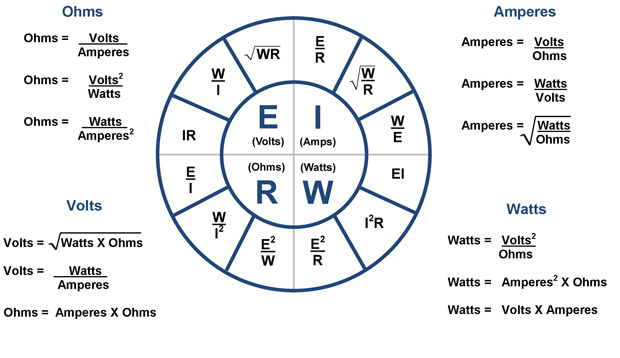
\includegraphics[scale=0.7]{imagenes/equation.jpg}
	\caption[Ley de Ohm y Watt.]{Ley de Ohm y Watt. Fuente \cite{calculadoraohm}.}
	\label{fig:formulaondas}
\end{figure}


\end{itemize}

\subsection{Módulo para mostrar información en la pantalla LCD}

Para mostrar información en una pantalla LCD no existen bibliotecas exclusivas diseñadas para el ESP8266 pero esta biblioteca \textit{LiquidCrystal\textunderscore I2C.h} diseñada para Arduino \cite{lcdgithub} nos permitirá mostrar la información que queramos sin ningún tipo de problema. Al estar compartiendo la conexión I2C con el conversor analógico digital tendremos que especificar en la creación del objeto la dirección de memoria de la pantalla LCD. 

Una vez creado el objeto tan solo tendremos que llamar a la función creada para mostrar la información deseada la cuál se le pasará a la función como argumentos:

\begin{listing}[style=consola, numbers=none]
	void imprimirLcd(double irms, double potencia){
		lcd.clear();
		lcd.print("irms: ");lcd.print(irms);lcd.print("A");
		lcd.setCursor(0,1);
		lcd.print("Potencia: ");lcd.print(potencia);lcd.print("W");
	}
\end{listing} 



\subsection{Módulo envío de información al servidor}

Para el envío de la información se ha decidido enviarla mediante HTTP (Hypertext Transfer Protocol), se trata de un protocolo de comunicación en red que hace posible la comunicación entre un cliente y un servidor mediante peticiones por parte del cliente y respuestas por parte del servidor \cite{httpinfo}. Para este proyecto vamos a utilizar el método de petición POST mediante el cuál seremos capaces de enviar la información que deseemos especificando la URL del servidor donde queramos enviar dicha información, cuado esa información sea recibida por el servidor se enviará una respuesta al cliente que generó la petición POST.  Gracias a la biblioteca \textit{ESP8266HTTPClient.h} \cite{httpclientgithub} una biblioteca para dispositivos IoT es posible realizar (entre otros métodos implementados en esta biblioteca) una petición POST de una manera muy sencilla en la placa ESP8266 en concreto gracias a la función:

\begin{listing}[style=consola, numbers=none]
	int POST(String payload);
\end{listing} 

A la hora de escoger en que formato enviar la información al servidor se ha escogido JSON (JavaScript Object Notation) que no es más que un formato para para realizar intercambio de datos. Haciendo uso de la biblioteca \textit{ArduinoJson.h} \cite{jsongithub} con la que podremos codificar arrays o incluso añadir valores al objeto creado directamente. 

Todo esto se realizará llamando a la función que se ha creado para hacer el código más legible. Pero la parte correspondiente únicamente a la codificación del JSON es la siguiente 

\begin{listing}[style=consola, numbers=none]
	StaticJsonBuffer<300> JSONbuffer;   //Declarar JSON buffer
	JsonObject& JSONencoder = JSONbuffer.createObject();
	
	JSONencoder["sensorType"] = "Power";
	Serial.println("irms dentro de mandarjson: ");Serial.println(irms);
	JsonArray& values = JSONencoder.createNestedArray("values"); //JSON array
	values.add(irms); //Aniadir valor al array
	values.add(potencia); //Aniadir valor al array
	
	JsonArray& valuesInfo = JSONencoder.createNestedArray("valuesInfo"); //JSON array
	valuesInfo.add("irmsnuevo"); //Aniadir valor al array
	valuesInfo.add("potencianueva"); //Aniadir valor al array
	
	char JSONmessageBuffer[300];
	JSONencoder.prettyPrintTo(JSONmessageBuffer, sizeof(JSONmessageBuffer));
	Serial.println(JSONmessageBuffer);


\end{listing} 




%
\chapter{Módulo servidor}
Para este proyecto se ha decidido crear un servidor propio con IP local. Es cierto que este servidor podría haberse alojado en algún hosting. Pero para asegurar la privacidad de los datos que publica el usuario de este monitor se ha decidido que lo mejor es alojar el servidor en una Raspberry Pi con IP local.

\section{Requisitos}
\subsection{Requisitos funcionales}

\begin{itemize}
	\item\textbf{RF1: } Ha de permitir al usuario consultar los consumos en un intervalo de fechas.
	\item\textbf{RF2: } Mostrar mediante una tabla los consumos ordenados por fecha y hora.
	\item\textbf{RF3: } En caso de mostrar una tabla muy extensa dividirla por páginas mediante un paginador.
	\item\textbf{RF4: } Mostrar la media de consumo durante las fechas especificadas por el usuario.
	\item\textbf{RF5: } Mostrar mediante un gráfico consumos del mes anterior y posterior al consultado por el usuario.
\end{itemize}

\subsection{Requisitos no funcionales}

\begin{itemize}
	\item\textbf{RNF1: } Hacer que el diseño de la web sea responsivo, es decir que se adapte a tamaños de pantalla diferentes para ajustarse a dispositivos móviles como smartphones o tablets o a ordenadores.
	\item\textbf{RNF2: } Persistencia de datos mediante una base de datos NoSql.
	\item\textbf{RNF3: } Se utilizarán tecnologías open source.
	\item\textbf{RNF4: } Garantizar la privacidad de los datos del usuario.
	\item\textbf{RNF4: } Compatibilidad con los navegadores.
\end{itemize}

\section{Backend}
La parte del Backend de la aplicación web está realizada con Flask \cite{Flask}. Se trata de un microframework para python que utiliza plantillas Jinja2 \cite{jinja2info}. Para una aplicación web pequeña como es el caso de la que se va a realizar para este proyecto nos ha parecido más apropiado utilizar este microframework ya que al contrario que otros framework como puede ser Django cuenta con con pocas características las cuales se pueden ir añadiendo mediante módulos los cuales en función de nuestras necesidades podremos ir añadiendo, sin embargo en un framework como Django \cite{Django} ya se incluyen todos estos componentes.

El motivo principal para escoger Flask frente a Django principalmente ha sido por el conocimiento previo que tenia adquirido en la asignatura desarrollo de aplicaciones para internet. También se había trabajado con Django en la asignatura infraestructura virtual pero en menor medida.

Para la persistencia de datos hemos utilizado bases de datos NoSQL más concretamente MongoDB, se trata de una base de datos orientada a documentos los datos se guardan en documentos BSON (una representación binaria de JSON) en lugar de en registros como ocurre en bases de datos convencionales. Esto permite introducir cualquier dato aunque se cambie el formato al contrario que en las bases de datos relacionales que es necesario seguir un esquema \cite{MongoDB}.

\section{Frontend}
Para realizar el frontend de la aplicación se han utilizado plantillas HTML 5 bootstrap para conseguir que el diseño de la web sea responsive. Al utilizar bootstrap conseguimos que el diseño de la web sea compatible con la mayoría de navegadores web \cite{Bootstrap}.
Se necesita además una herramienta open source para realizar las gráficas de consumo. Para ello se ha utilizado la herramienta Higcharts la cuál nos permite realizar gráficas utilizando JavaScript.

\section{Servidor}
Para alojar la aplicación web diseña para este proyecto no es necesario un servidor con demasiada potencia por lo tanto con alojar la web en una Raspberry Pi nos será más que suficiente.

\subsection{Sistema Operativo}

Como vamos a utilizar la Raspberry como servidor instalaremos un sistema operativo sin interfaz gráfica en concreto Raspbian Jessie Lite. Para instalar el sistema operativo en la tarjeta micro SD que introduciremos en la Raspberry tan solo tendremos que flashear la imagen que nos descargaremos de la web oficial de raspberry \cite{raspbianoficial}. Para flashear la imagen en la SD existen múltiples programas pero en mi caso he elegido utilizar Win32 disk imager \cite{Win32} un sencillo software open source disponible para múltiples plataformas que nos permitirá flashear la imagen en la tarjeta micro SD muy fácilmente. Hemos de tener en cuenta que previamente la tarjeta micro SD tendrá que estar formateada para lo cuál nos servirá cualquier software open source de los que están disponibles.

\subsection{Aprovisionamiento }
Para facilitar que cualquier persona interesada en el proyecto pueda montar de la forma más sencilla posible el servidor tan solo tendrá que descargarse mi repositorio de GitHub \url{https://github.com/Miguelmoral/ESP8266-energy-monitor}, los pasos a seguir para su descarga y puesta en funcionamiento son bastante sencillos \cite{repoESP}:

\begin{enumerate}
	\item\textbf{Instalar git: } Para poder descargar el repositorio de GitHub será necesaria la instalación de git en nuestra máquina con el comando:
	 \begin{listing}[style=consola, numbers=none]
	 	$ sudo apt-get update
		$ sudo apt-get install git
	\end{listing}
	\item\textbf{Descargar repositorio: } Una vez tenemos instalado git podremos descargar el repositorio introduciendo:
	
	\begin{listing}[style=consola, numbers=none]
	$ sudo git clone https://github.com/Miguelmoral/ESP8266-energy-monitor	
	\end{listing}
	
	\item\textbf{Instalar \textit{requirements}: } Una vez descargado este repositorio en el cuál se incluye todo lo necesario para el correcto funcionamiento del servidor el usuario tendrá que ejecutar el comando 
	
	\begin{listing}[style=consola, numbers=none]
		$ cd ESP8266-energy-monitor
		$ sudo make install
	\end{listing} 
		
\end{enumerate}

\subsection{Iniciar aplicación web }
El \textit{makefile} incluye además otro comando que permite directamente la ejecución de la aplicación web en el servidor, hay que tener en cuenta que para que este comando funcione previamente tendremos que haber realizado los pasos explicados anteriormente.

\begin{listing}[style=consola, numbers=none]
	$ make ejecutar
\end{listing} 

Al tratarse de una Raspberry Pi la cuál no dispone de pantalla sería interesante hacer que se ejecute automáticamente la aplicación web cada vez que arranquemos el sistema. Existen varias formas de conseguirlo \cite{rc.local}:

\begin{enumerate}
	\item Modificando el archivo rc.local.
	\item Modificando el archivo .bashrc.
	\item Añadir el \textit{script} o comandos que se quieran ejecutar al directorio /etc/init.d. 
	\item Utilizando los archivos systemd.
	\item Mediante el demonio cron. Tendremos que añadir los script que queramos ejecutar en el fichero crontab y especificar cuando queramos que se ejecuten. 
\end{enumerate}

 Para este proyecto se va a modificar el archivo rc.local de la máquina. Tan solo tendremos que abrir este archivo con un editor de textos con permisos root para poder editarlo e incluir antes de exit 0 el comando que queramos que ejecute la máquina cada vez que se encienda en nuestro caso.

Abriremos un editor de textos para modificar el archivo rc.local con

\begin{listing}[style=consola, numbers=none]
	$ sudo nano rc.local
\end{listing} 

Y añadiremos la orden 

\begin{listing}[style=consola, numbers=none]
$ sudo python /home/pi/ESP8266-energy-monitor/web/main.py &
\end{listing} 

Quedándose el archivo rc.local de esta forma \ref{fig:rc.local}

\begin{figure}[H]
	\centering
	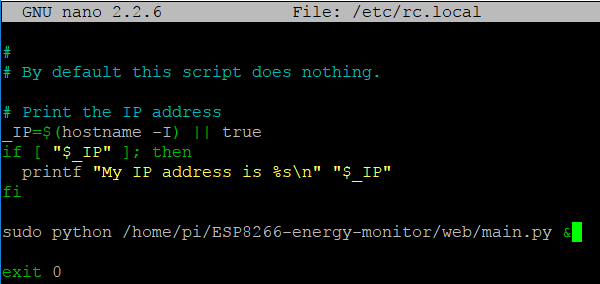
\includegraphics{imagenes/iniciaraplicacionweb2.png}
	\caption{rc.local Raspberry Pi}
	\label{fig:rc.local}
\end{figure}

\subsection{IP estática Raspberry }
Establecer una IP estática en la Raspberry no es totalmente necesario para el proyecto ya que podría funcionar perfectamente con una IP dinámica, pero por comodidad es preferible establecer una IP estática.

Para que el ESP8266 pueda mandar la información siempre a la misma IP y no tener que modificar el código del firmare cada vez que la Raspberry cambie de IP vamos a hacer que la IP de la Raspberry que por defecto es dinámica pase a ser estática de esta forma esta IP será siempre la misma la cuál le asignaremos nosotros modificando el archivo.

Tendremos que consultar algunos valores sobre nuestra conexión antes de modificar el archivo /etc/network/interfaces \cite{staticip}. Para ello utilizaremos el comando :
\begin{listing}[style=consola, numbers=none]
	$ netstat -nr 
\end{listing} 

Una vez sabemos cuál es nuestro broadcast range, subnet mask, gateway y destination podremos modificar el archivo /etc/network/interfaces de nuestra Raspberry para establecer una IP fija. Dependiendo de los valores que nos de dependiendo de la configuración de nuestra conexión tendremos que cambiar algunos datos a la hora de modificar este archivo pero en mi caso obtendríamos algo como lo que vemos en la imagen \ref{fig:confip}:

\begin{figure}[H]
	\centering
	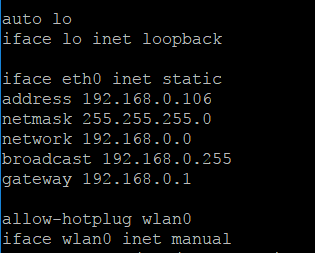
\includegraphics{imagenes/staticipconf.png}
	\caption{Configuración /etc/network/interfaces}
	\label{fig:confip}
\end{figure}


\subsection{Aspecto final de la página}

Tendremos una simple página de inicio donde podremos seleccionar de que fecha a que fecha queremos visualizar los datos:

\begin{figure}[H]
	\centering
	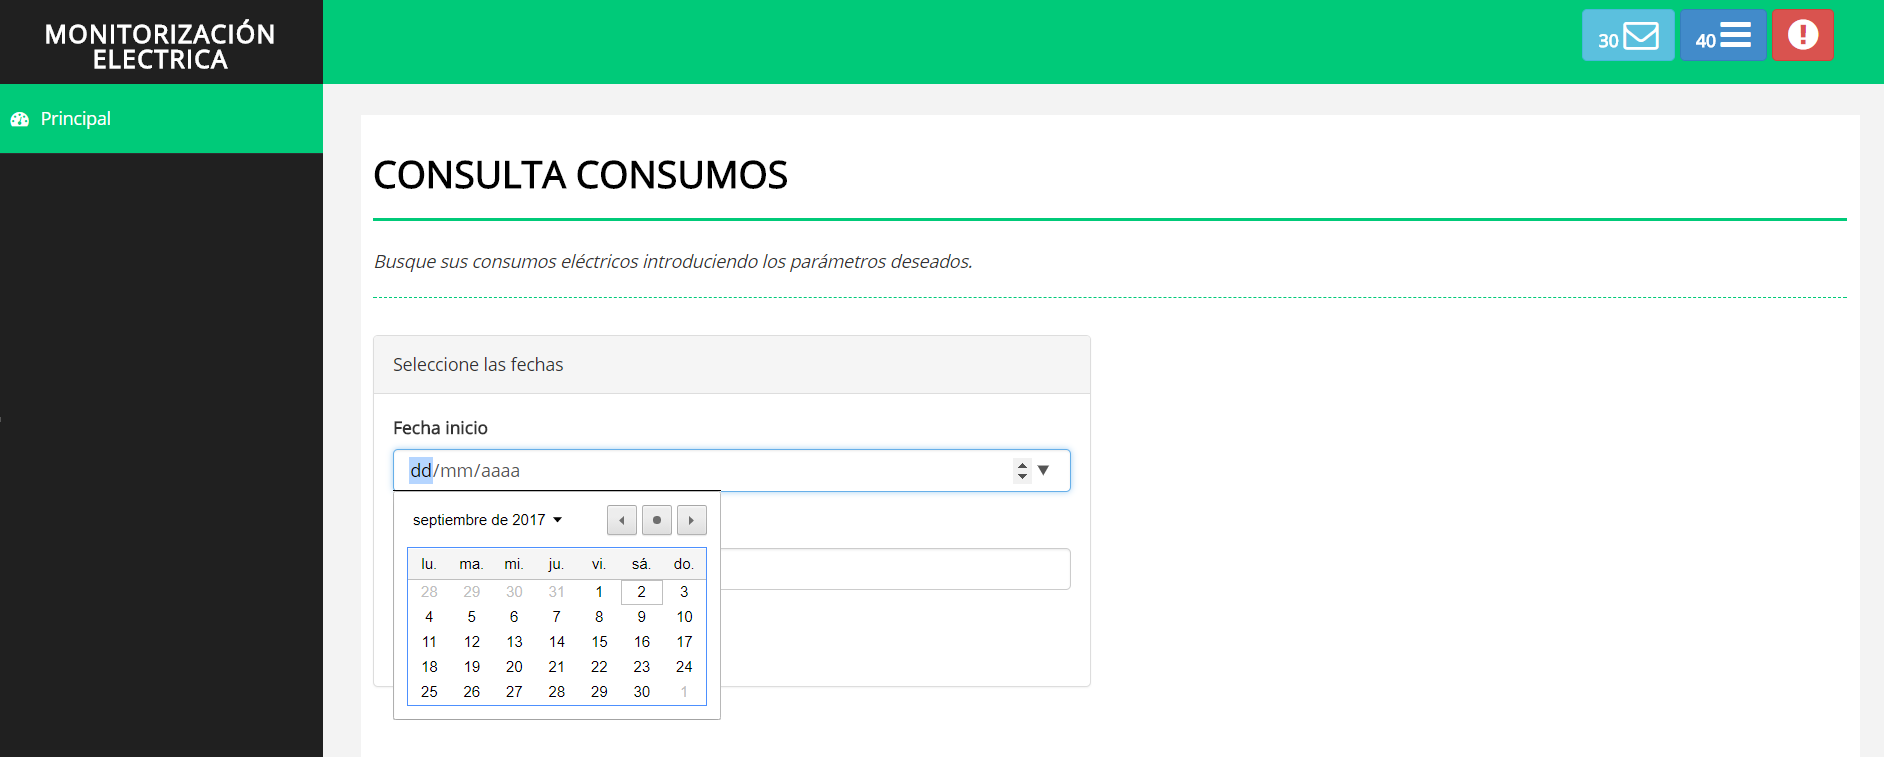
\includegraphics[scale=0.4]{imagenes/principalfecha.png}
	\caption{Página principal}
	\label{fig:principalweb}
\end{figure}

Al introducir las fechas veremos una tabla con los datos correspondientes a las fechas introducidas, un apartado que nos muestra la media tanto del irms como de la potencia consumida y una gráfica correspondiente a las medias de el mes anterior al consultado y el siguiente. En la gráfica mostrada tanto el mes siguiente como el anterior sale a 0 ya que durante esos meses no se recogieron muestras. En la gráfica (\ref{fig:tablaconsumos}) podemos ver los resultados de medir una bombilla de 60 W durante un periodo de tiempo. El paginador nos mostrará 10 entradas por página de esta forma se podrán visualizar los datos de una forma más clara que si se mostraran sin paginador. Además tendremos una gráfica que nos irá mostrando los últimos consumos que reciva el servidor (\ref{fig:grafultimos})

\begin{figure}[H]
	\centering
	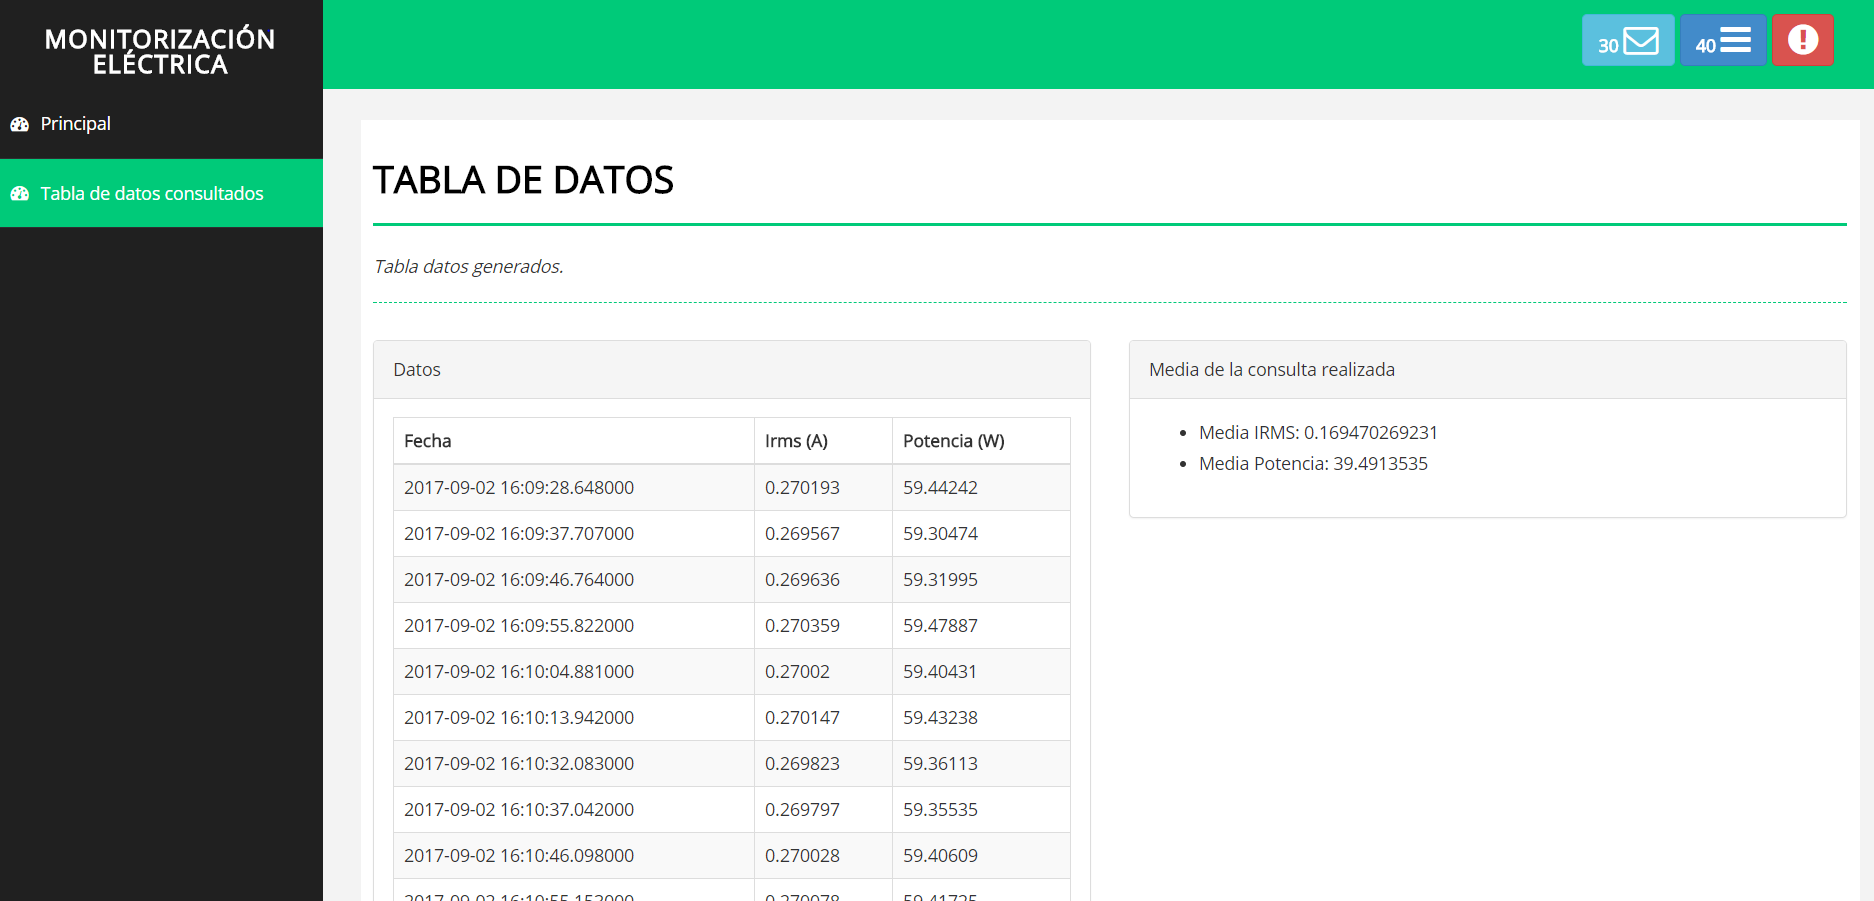
\includegraphics[scale=0.4]{imagenes/webbombillaconstante.png}
	\caption{Tabla de datos}
	\label{fig:tablaconsumos}
\end{figure}

\begin{figure}[H]
	\centering
	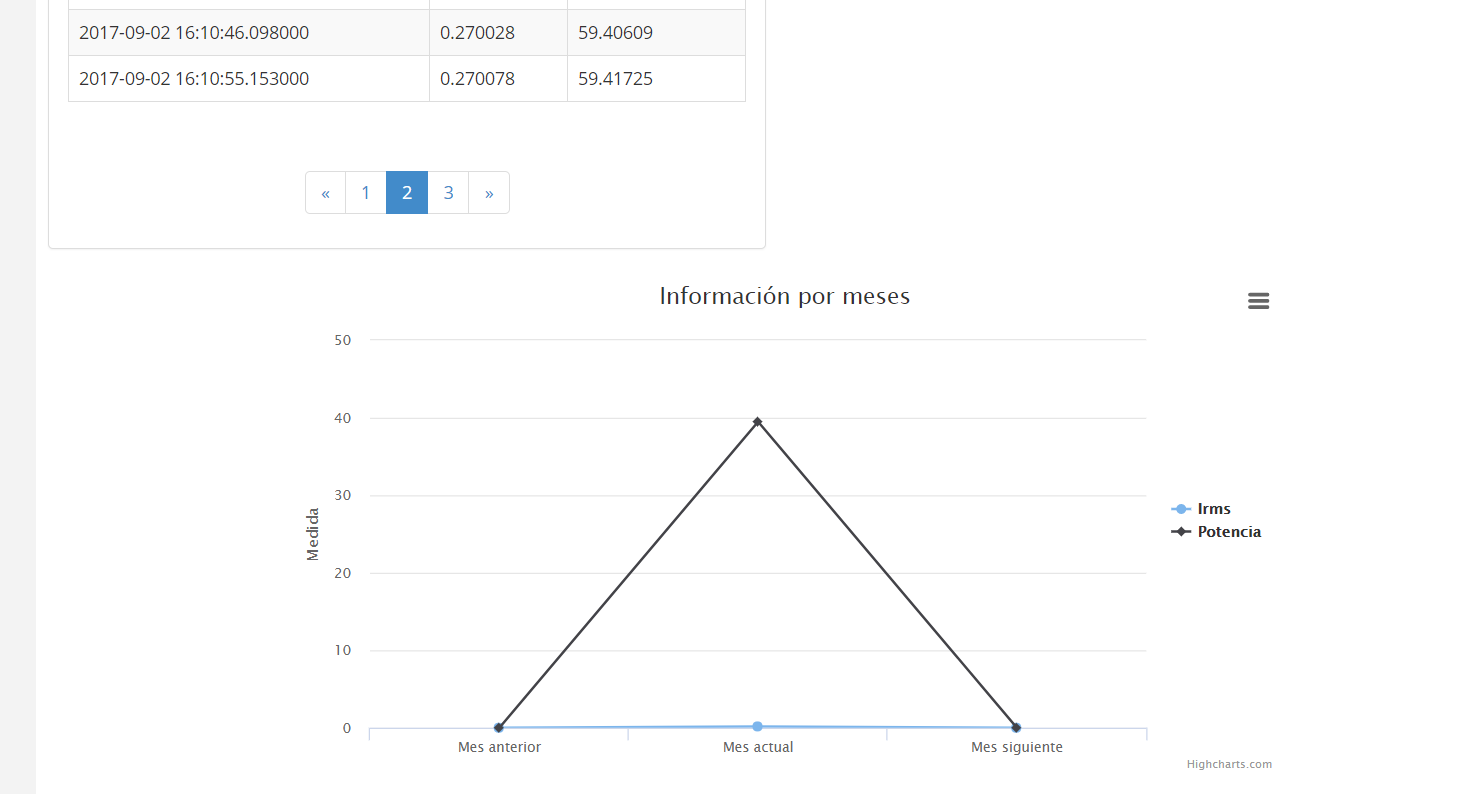
\includegraphics[scale=0.4]{imagenes/graficabombilla.png}
	\caption{Gráfica mensual}
	\label{fig:grafmensual}
\end{figure}

\begin{figure}[H]
\centering
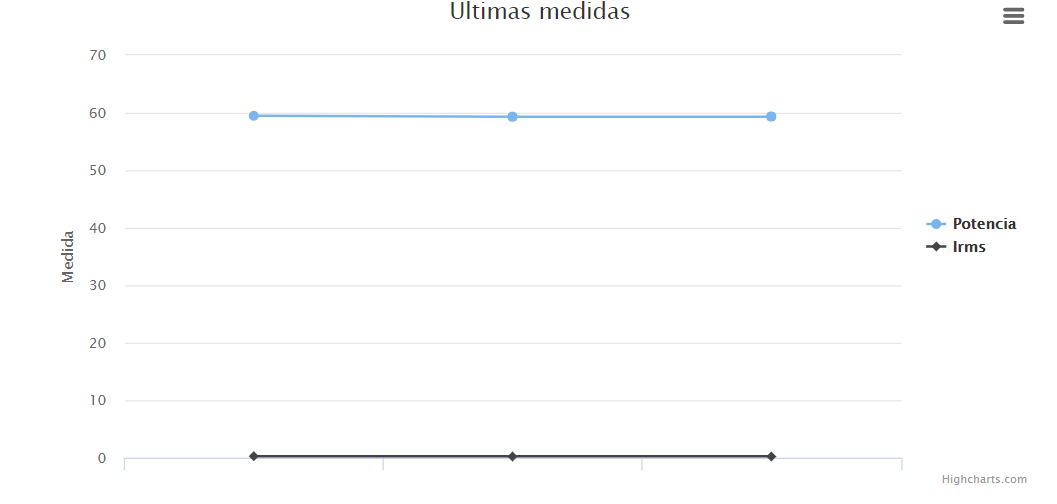
\includegraphics[scale=0.5]{imagenes/grafultima.png}
\caption{Gráfica ultimos consumos}
\label{fig:grafultimos}
\end{figure}


%
\chapter{Pruebas}
En el siguiente capítulo se expondrán algunas de las pruebas realizadas hasta que se consiguió finalmente realizar un diseño funcional:

\begin{itemize}
	\item \textbf{Prueba 1:} En este primera prueba se intentará hacer funcionar un circuito simple, en concreto el primer prototipo especificado en en el capítulo 4 (\ref{fig:protoboardv1}). Simplemente se quiere comprobar que todo funciona como debería por lo que en el firmware se cargará tan solo un programa simple que saque por la salida serial al ordenar los datos recogidos de el conversor analógico digital sin realizar ningún tipo de cálculo.
	
	\begin{table}[H]
		\begin{center}
			\begin{tabular}{|l|l|}
				\hline
				Número de prueba &  1 \\ \hline 
				Objetivo de la prueba &  Comprobar funcionamiento del prototipo (\ref{fig:protoboardv1}).\\ \hline 
				Procedimientos a llevar a cabo &  \makecell[l]{\tabitem Montar diseño del circuito en la protoboard. \\ \tabitem Programar un firmware sencillo.
				\\ \tabitem Flashear el firmware en la placa NodeMCU.
				\\ \tabitem Visualizar resultados en la pantalla del ordenador.}
				 \\ \hline 
				Resultado deseado &  \makecell[l]{Visualizar resultados lógicos dependiendo \\ de que aparato esté conectado al sensor.} \\ \hline 
				Resultado obtenido &  \makecell[l]{Los resultados que vemos en pantalla son \\ siempre 0 o demasiado cercanos al 0, además son siempre \\ iguales independientemente de la electricidad que esté \\ consumiendo el aparato en cada momento.} \\ \hline  
				Estado de la prueba &  \textbf{Error.} \\ \hline 
				Posibles soluciones &  \makecell[l]{Diseñar otro prototipo con una entrada de energía \\diferente al micro USB. } \\ \hline 

			\end{tabular}
			\caption{Prueba 1.}
			\label{tabla:prueba1}
		\end{center}
	\end{table}

	\vspace{2.5cm}

	\item \textbf{Prueba 2:} Para intentar solucionar el error de la prueba 1 se va a probar un segundo prototipo (\ref{fig:protoboardv2}) alimentado a través del jack de corriente para ver si el problema era que le entraba un voltaje menor al necesario utilizando la entrada micro USB propia de la placa NodeMCU.

	\begin{table}[H]
	\begin{center}
		\begin{tabular}{|l|l|}
			\hline
			Número de prueba &  2 \\ \hline 
			Objetivo de la prueba &  Comprobar funcionamiento del prototipo (\ref{fig:protoboardv2}).\\ \hline 
			Procedimientos a llevar a cabo &  \makecell[l]{\tabitem Montar diseño del circuito en la protoboard. \\ \tabitem Programar un firmware que envíe los datos \\ a un servidor.
				\\ \tabitem Flashear el firmware en la placa NodeMCU.
				\\ \tabitem Visualizar resultados que se muestran en el servidor.}
			\\ \hline 
			Resultado deseado &  \makecell[l]{Visualizar resultados lógicos dependiendo \\ de que aparato esté conectado al sensor.} \\ \hline 
			Resultado obtenido &  \makecell[l]{La placa NodeMCU ha resultado dañada al \\ utilizar un cargador cuya salida es corriente alterna.} \\ \hline 
			Estado de la prueba &  \textbf{Error.} \\ \hline 
			Posibles soluciones &  \makecell[l]{Utilizar un cargador cuya salida sea corriente continua.} \\ \hline 
			
		\end{tabular}
		\caption{Prueba 2.}
		\label{tabla:prueba2}
		\end{center}
	\end{table}

	\vspace{10cm}

	\item \textbf{Prueba 3:} Para intentar solucionar el error de la prueba 1 se va a probar un segundo prototipo (\ref{fig:protoboardv2}) alimentado a través del jack de corriente para ver si el problema era que le entraba un voltaje menor al necesario utilizando la entrada micro USB propia de la placa NodeMCU.



	\begin{table}[H]
		\begin{center}
			\begin{tabular}{|l|l|}
				\hline
				Número de prueba &  2 \\ \hline 
				Objetivo de la prueba &  Comprobar funcionamiento del prototipo (\ref{fig:protoboardv2})\\ \hline 
				Procedimientos a llevar a cabo &  \makecell[l]{\tabitem Montar diseño del circuito en la protoboard. \\ \tabitem Programar un firmware que envíe los datos \\ a un servidor.
					\\ \tabitem Flashear el firmware en la placa NodeMCU.
					\\ \tabitem Visualizar resultados que se muestran en el servidor.}
				\\ \hline 
				Resultado deseado &  \makecell[l]{Visualizar resultados lógicos dependiendo \\ de que aparato esté conectado al sensor.} \\ \hline 
				Resultado obtenido &  \makecell[l]{Los resultados que vemos en pantalla son \\ siempre 0 o demasiado cercanos al 0, además son siempre \\ iguales independientemente de la electricidad que esté \\ consumiendo el aparato en cada momento.} \\ \hline 
				Estado de la prueba &  \textbf{Error.} \\ \hline 
				Posibles soluciones &  \makecell[l]{Comprobar que el sensor de corriente \\ funcione correctamente. } \\ \hline 
				
			\end{tabular}
			\caption{Prueba 2.}
			\label{tabla:prueba2}
		\end{center}
	\end{table}

	\vspace{8.5cm}
	
	\item \textbf{Prueba 4:} Se realizará una prueba simple conectando el sensor a un Arduino utilizando la comunicación serie para ver en el ordenador si el sensor está funcionando correctamente o tiene algún tipo de fallo y este es el motivo por el cuál las medidas que estamos tomando son tan cercanas al 0 y no varían en función de la energía que consume en cada momento el aparato al que está conectado el sensor.
	
		\begin{table}[H]
		\begin{center}
			\begin{tabular}{|l|l|}
				\hline
				Número de prueba &  4 \\ \hline 
				Objetivo de la prueba &  Comprobar funcionamiento del sensor de corriente. \\ \hline 
				Procedimientos a llevar a cabo &  \makecell[l]{\tabitem Montar diseño del circuito en el propio Arduino. \\ \tabitem Programar un firmware sencillo.
					\\ \tabitem Flashear el firmware en el Arduino.
					\\ \tabitem Visualizar resultados en la pantalla del ordenador.}
				\\ \hline 
				Resultado deseado &  \makecell[l]{Visualizar resultados lógicos dependiendo \\ de que aparato esté conectado al sensor.} \\ \hline 
				Resultado obtenido &  \makecell[l]{Los resultados que vemos en pantalla son \\ siempre 0 o demasiado cercanos al 0, además son siempre \\ iguales independientemente de la electricidad que esté \\ consumiendo el aparato en cada momento.} \\ \hline 
				Errores &  \makecell[l]{Los resultados obtenidos de la medición no son correctos \\ ya que son siempre iguales independientemente de la \\electricidad que esté consumiendo el aparato en\\ cada momento.} \\ \hline 
				Estado de la prueba &  \textbf{Error.} \\ \hline 
				Posibles soluciones &  \makecell[l]{Diseñar un prototipo con un amplificador \\ para conseguir valores mayores. } \\ \hline 
				
			\end{tabular}
			\caption{Prueba 4.}
			\label{tabla:prueba4}
		\end{center}
	\end{table}

	\vspace{7cm}

	\item \textbf{Prueba 5:} Para comprobar si el problema de las mediciones viene dado por que la señal que estamos midiendo es demasiado baja. El diseño de este circuito corresponde con el visto en el capítulo 4 (\ref{fig:protoboardv3}).

	\begin{table}[H]
		\begin{center}
			\begin{tabular}{|l|l|}
				\hline
				Número de prueba &  5 \\ \hline 
				Objetivo de la prueba &  Comprobar funcionamiento del prototipo (\ref{fig:protoboardv3}). \\ \hline 
				Procedimientos a llevar a cabo &  \makecell[l]{\tabitem Montar diseño del circuito en la protoboard. \\ \tabitem Programar un firmware que envíe los datos \\ a un servidor.
				\\ \tabitem Flashear el firmware en la placa NodeMCU.
				\\ \tabitem Visualizar resultados que se muestran en el servidor.}
				\\ \hline 
				Resultado deseado &  \makecell[l]{Visualizar resultados lógicos dependiendo \\ de que aparato esté conectado al sensor.} \\ \hline 
				Resultado obtenido &  \makecell[l]{Los resultados obtenidos de la medición no son correctos \\ ya que son siempre iguales independientemente de la \\electricidad que esté consumiendo el aparato en\\ cada momento.} \\ \hline 
				Estado de la prueba &  \textbf{Error} \\ \hline 
				Posibles soluciones &  \makecell[l]{Colocar el sensor de corriente rodeando tan solo \\ uno de los cables (una fase) que tiene la manguera.} \\ \hline 
				
			\end{tabular}
			\caption{Prueba 5.}
			\label{tabla:prueba5}
		\end{center}
	\end{table}
	
	\vspace{9.5cm}
	
	\item \textbf{Prueba 6:} Se probará de nuevo el prototipo (\ref{fig:protoboardv2}) pero en esta ocasión el sensor de corriente se colocará al rededor de tan solo uno de los tres cables (una fase) de la manguera que contiene los tres cables.
	
	\begin{table}[H]
		\begin{center}
			\begin{tabular}{|l|l|}
				\hline
				Número de prueba &  6 \\ \hline 
				Objetivo de la prueba &  Comprobar funcionamiento del prototipo (\ref{fig:protoboardv2}). \\ \hline 
				Procedimientos a llevar a cabo &  \makecell[l]{\tabitem Montar diseño del circuito en la protoboard. \\ \tabitem Programar un firmware para visualizar \\ los datos por pantalla.
					\\ \tabitem Flashear el firmware en la placa NodeMCU.
					\\ \tabitem Visualizar resultados que se muestran en la pantalla.}
				\\ \hline 
				Resultado deseado &  \makecell[l]{Visualizar resultados lógicos dependiendo \\ de que aparato esté conectado al sensor.} \\ \hline 
				Resultado obtenido &  \makecell[l]{Los resultados son lógicos con respecto a los consumos \\ que está haciendo el aparato al que está conectado \\ el sensor.} \\ \hline 
				Estado de la prueba &  \textbf{Correcto.} \\ \hline 
				Posibles soluciones &  \makecell[l]{} \\ \hline 
				
			\end{tabular}
			\caption{Prueba 6.}
			\label{tabla:prueba6}
		\end{center}
	\end{table}
	
	\vspace{10.5cm}
	
	\item \textbf{Prueba 7:} Comprobación del correcto funcionamiento del prototipo (\ref{fig:protoboardv4}) con un firmware que calcule el irms y que muestre la información a través de la pantalla LCD. Además se comparará la información obtenida utilizando el prototipo con la obtenida utilizando un sensor comercial.
	
	\begin{table}[H]
		\begin{center}
			\begin{tabular}{|l|l|}
				\hline
				Número de prueba &  7 \\ \hline 
				Objetivo de la prueba &  Comprobar funcionamiento del prototipo (\ref{fig:protoboardv4}). \\ \hline 
				Procedimientos a llevar a cabo &  \makecell[l]{\tabitem Montar diseño del circuito en la protoboard. \\ \tabitem Programar un firmware para visualizar \\ los datos por pantalla.
					\\ \tabitem Flashear el firmware en la placa NodeMCU.
					\\ \tabitem Visualizar resultados que se muestran en la pantalla.
					\\ \tabitem Comparar con los datos recogidos por el \\ sensor comercial.
				}
				\\ \hline 
				Resultado deseado &  \makecell[l]{Visualizar los mismos resultados que los \\ que obtendríamos utilizando el sensor comercial.} \\ \hline 
				Resultado obtenido &  \makecell[l]{Los resultados son lógicos con respecto \\ a los consumos que está haciendo el aparato al que está \\ conectado \\ el sensor, pero no son iguales a los datos \\ que visualizamos en el sensor comercial.} \\ \hline 
				Estado de la prueba &  \textbf{Error.} \\ \hline 
				Posibles soluciones &  \makecell[l]{Calibrar el sensor.} \\ \hline 
				
			\end{tabular}
			\caption{Prueba 7.}
			\label{tabla:prueba7}
		\end{center}
	\end{table}

	\vspace{8cm}
	
	\item \textbf{Prueba 8:} Comprobación del correcto funcionamiento del prototipo (\ref{fig:protoboardv4}) con un firmware que calcule el irms y que muestre la información a través de la pantalla LCD. Además se comparará la información obtenida utilizando el prototipo con la obtenida utilizando un sensor comercial. Con la diferencia de que en esta ocasión se añadirá en el firmware una variable que nos permitirá calibrar el sensor.

	\begin{table}[H]
		\begin{center}
			\begin{tabular}{|l|l|}
				\hline
				Número de prueba &  8 \\ \hline 
				Objetivo de la prueba &  Comprobar funcionamiento del prototipo (\ref{fig:protoboardv4}). \\ \hline 
				Procedimientos a llevar a cabo &  \makecell[l]{\tabitem Montar diseño del circuito en la protoboard. \\ \tabitem Programar un firmware para visualizar \\ los datos por pantalla.
					\\ \tabitem Flashear el firmware en la placa NodeMCU.
					\\ \tabitem Visualizar resultados que se muestran en la pantalla.
					\\ \tabitem Comparar con los datos recogidos por el \\ sensor comercial.
				}
				\\ \hline 
				Resultado deseado &  \makecell[l]{Visualizar los mismos resultados que los \\ que obtendríamos utilizando el sensor comercial.} \\ \hline 
				Resultado obtenido &  \makecell[l]{La información visualizada utilizando \\el prototipo coincide con la que observamos en el sensor \\ comercial. } \\ \hline 
				Estado de la prueba &  \textbf{Correcto.} \\ \hline 
				Posibles soluciones &  \makecell[l]{} \\ \hline 
				
			\end{tabular}
			\caption{Prueba 8.}
			\label{tabla:prueba8}
		\end{center}
	\end{table}

	\item \textbf{Prueba 9:} Revisión del firmware para poder mandar los datos en formato JSON a un servidor.

	\begin{table}[H]
		\begin{center}
			\begin{tabular}{|l|l|}
				\hline
				Número de prueba &  9 \\ \hline 
				Objetivo de la prueba &  Enviar la información a un servidor. \\ \hline 
				Procedimientos a llevar a cabo &  \makecell[l]{\tabitem Adaptar el firmware para enviar datos \\ especificando la IP del servidor. 
				\\ \tabitem Flashear el firmware en la placa NodeMCU.
				\\ \tabitem Comprobar que los datos se reciben de forma correcta \\ en el servidor.
				}
				\\ \hline 
				Resultado deseado &  \makecell[l]{Los datos se reciben en el servidor sin ningún \\ tipo de problema.} \\ \hline 
				Resultado obtenido &  \makecell[l]{El servidor recibe los datos de la manera esperada.} \\ \hline 
				Estado de la prueba &  \textbf{Correcto.} \\ \hline 
				Posibles soluciones &  \makecell[l]{} \\ \hline 
				
			\end{tabular}
			\caption{Prueba 9.}
			\label{tabla:prueba9}
		\end{center}
	\end{table}
	
\end{itemize}
%
\chapter{Experimentación}

En este capítulo se recogerán algunos experimentos realizados para cerciorarnos de que las medidas recogidas gracias al aparato diseñado se corresponde a medidas reales.

\section{Comparativas con aparatos reales}

Para poder calibrar el dispositivo y ver si las medidas recogidas son adecuadas lo que se ha hecho ha sido comparar las mediciones de distintos aparatos utilizando un medidor de consumos eléctricos del mercado, en concreto el modelo más simple de efergy el cual se encuentra entre los dispositivos que podemos encontrar en el mercado analizados en el capítulo 1.

Una vez calibrado el dispositivo podemos ver en la siguiente tabla que los resultados obtenidos mediante el monitor de energía comercial y el que hemos diseñado nosotros las diferencias son mínimas:

\begin{table}[H]
	\begin{center}
		\begin{tabular}{|l||l|l|}
			\hline
			Aparato a medir & Medida Efergy & Medida con nuestro sensor \\
			\hline \hline
			Bombilla 40 W & 41.2 W & 41.14
 W \\ \hline
			Bombilla 60 W & 59.8 W & 59.76

 W \\ \hline
			Play Station & 47 W & 51.48
 W \\ \hline
			Ventilador & 35.4 W & 35.32
 W \\ \hline
			TV & 16.7 W & 17.52
 W \\ \hline
			Secador a plena potencia & 1902 W & 1910.52
 W \\ \hline
			Secador media potencia & 983 W & 984.58
 W \\ \hline
			Secador baja potencia & 530 W & 534.23
 W \\ \hline
		\end{tabular}
		\caption{Comparación consumos.}
		\label{tabla:consumos aparatos}
	\end{center}
\end{table}

\section{Prueba consumo constante}

En este apartado comprobaremos que el aparato funciona correctamente midiendo el consumo constante durante un periodo de tiempo de una bombilla de 60 W este consumo se empezará a medir empezando con la bombilla apagada y finalmente con la bombilla apagada también por ese motivo la primera y última muestra son 0. Estas muestras se han recogido por comodidad conectando la placa directamente al puerto USB del ordenador y abriendo el monitor serie (\ref{fig:monitorserial}). Podremos ver estos resultados más claramente haciendo una gráfica en una hoja de cálculo (\ref{fig:graficobombilla}). 

\begin{figure}[H]
	\centering
	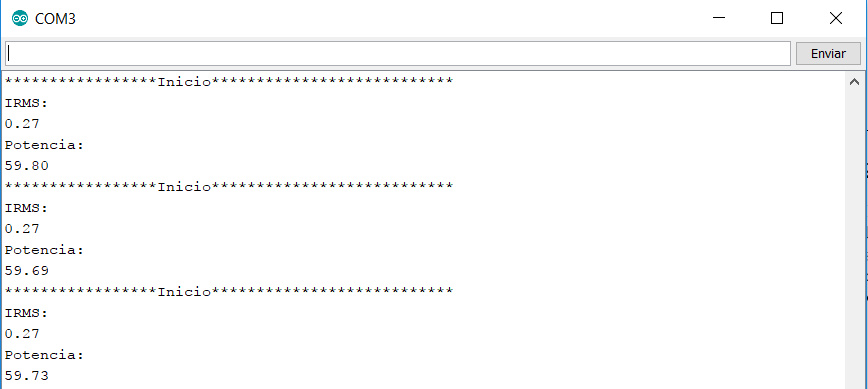
\includegraphics[scale=0.5]{imagenes/arduinoidemuestras.png}
	\caption{Monitor serial Arduino IDE.}
	\label{fig:monitorserial}
\end{figure}

\begin{figure}[H]
	\centering
	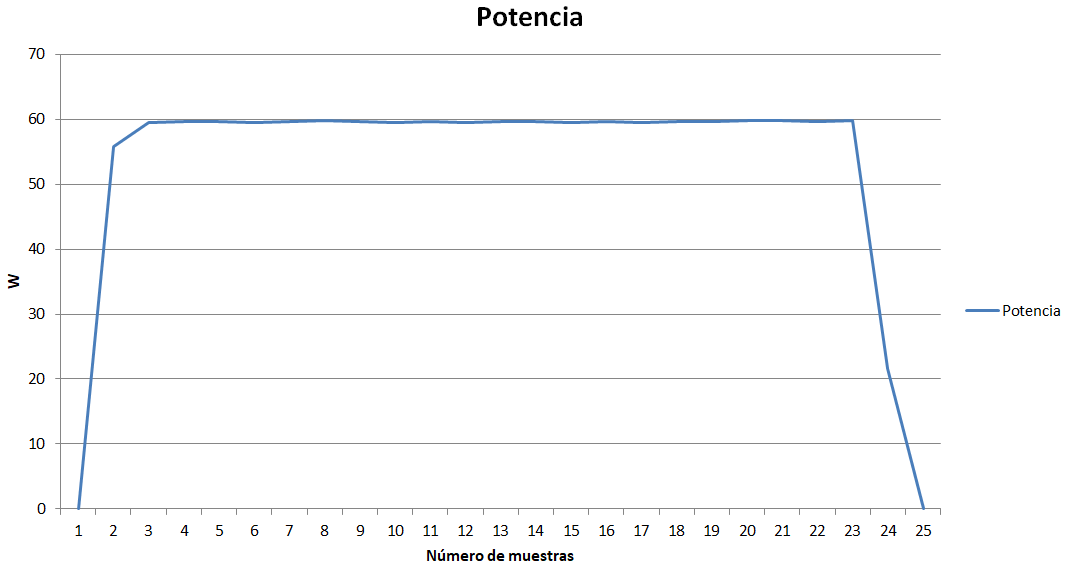
\includegraphics[scale=0.5]{imagenes/graficobombilla.png}
	\caption{Gráfico muestras recogidas.}
	\label{fig:graficobombilla}
\end{figure}

\section{Prueba con un electrodoméstico real}

Para esta prueba se ha conectado el sensor a un congelador y se han recogido medidas durante la noche obteniendo los siguientes resultados (\ref{fig:graficocongelador}). Además podemos observar como justo en el momento en el que el compresor del congelador vuelve a conectarse (Cuando detecta que ha perdido demasiada temperatura) el consumo se dispara ya que al volver a conectarse es cuando más energía consume.

\begin{figure}[H]
	\centering
	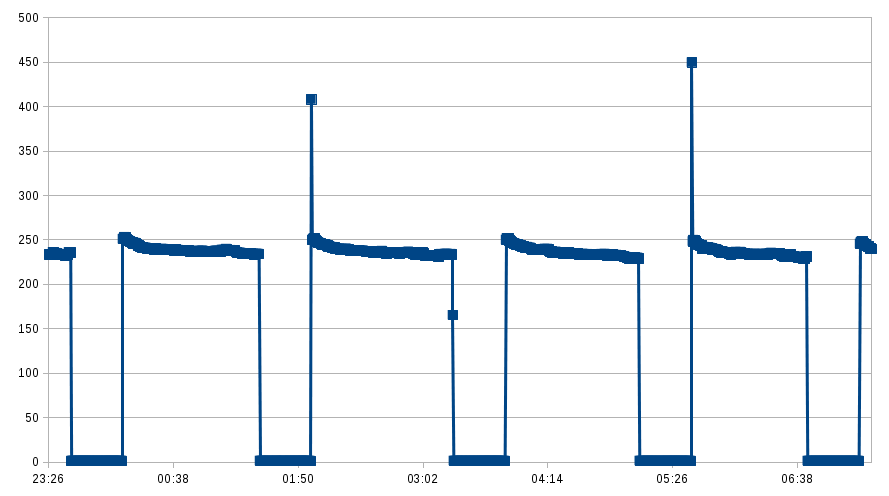
\includegraphics[scale=0.5]{imagenes/graficoFrigo.png}
	\caption{Muestras recogidas congelador.}
	\label{fig:graficocongelador}
\end{figure}

 Si analizamos los resultados más en detalle vemos que donde se produce un cambio significativo de la potencia registrada corresponde al tiempo que el compresor del congelador está activo y el tiempo que está apagado siempre es el mismo, como podemos ver con estos datos obtenidos directamente:

\begin{table}[H]
	\centering
	\begin{tabular}{|l|l|l|c|}
		\hline
		Hora                     & Medida   & Estado & \multicolumn{1}{l|}{Duración} \\ \hline \hline
		31/08/2017  23:39:12  AM & 1.23     & Off    & \multirow{2}{*}{0:29}         \\ \cline{1-3}
		01/09/2017 0:08          & 1.20     & Off    &                               \\ \hline
		01/09/2017 0:08          & 250.90   & On     & \multirow{2}{*}{1:35}         \\ \cline{1-3}
		01/09/2017 1:27          & 234.00   & On     &                               \\ \hline
		01/09/2017 1:27          & 1.21     & Off    & \multirow{2}{*}{0:30}         \\ \cline{1-3}
		01/09/2017 1:57          & 1.19     & Off    &                               \\ \hline
		01/09/2017 1:57          & 408.01 W & On     & \multirow{2}{*}{1:22}         \\ \cline{1-3}
		01/09/2017 3:19          & 165.26 W & On     &                               \\ \hline
		01/09/2017 3:19          & 1.20 W   & Off    & \multirow{2}{*}{0:30}         \\ \cline{1-3}
		01/09/2017 3:49          & 1.19 W   & Off    &                               \\ \hline
		01/09/2017 3:49          & 250.04 W & On     & \multirow{2}{*}{1:17}         \\ \cline{1-3}
		01/09/2017 5:06          & 229.31 W & On     &                               \\ \hline
		01/09/2017 5:07          & 1.20 W   & Off    & \multirow{2}{*}{0:29}         \\ \cline{1-3}
		01/09/2017 5:36          & 1.19 W   & Off    &                               \\ \hline
		01/09/2017 5:37          & 449.66 W & On     & \multirow{2}{*}{1:06}         \\ \cline{1-3}
		01/09/2017 6:43          & 231.48 W & On     &                               \\ \hline
		01/09/2017 6:44          & 1.19 W   & Off    & \multirow{2}{*}{0:29}         \\ \cline{1-3}
		01/09/2017 7:13          & 1.18 W   & Off    &                               \\ \hline
		01/09/2017 7:14          & 245.68 W & On     & \multicolumn{1}{l|}{}         \\ \hline
	\end{tabular}

	\caption{Tabla datos}
\label{fig:datoscongelador}
\end{table}
Todos estos resultados han sido obtenidos sin abrir en ningún momento la puerta del congelador. Pero en caso de que se abra la puerta del congelador se perderá frío y tendrá que conectar el compresor antes como podemos ver en esta otra gráfica (\ref{fig:abriendopuerta}) en la que justo en el momento en el que el compresor del congelador se apagó, se dejó abierta la puerta hasta que a los 3 minutos el congelador encendió de nuevo el compresor.

\begin{figure}[H]
	\centering
	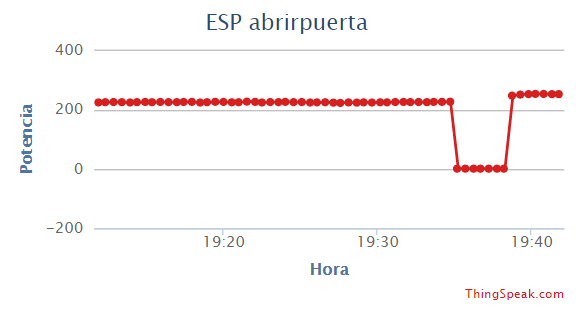
\includegraphics[scale=0.7]{imagenes/abriendopuerta.png}
	\caption{Muestras recogidas congelador.}
	\label{fig:abriendopuerta}
\end{figure}

\section{Posibilidades de explotación de un dispositivo como el presentado}

Como hemos visto gracias a la prueba anterior realizada en el congelador gracias a los patrones de consumo que observamos podemos determinar que electrodoméstico o dispositivo es el que está realizando esos consumos. Pero este estudio de los datos de consumo recogidos podría ir a más ya que como hemos observado es posible incluso determinar cuando el usuario ha abierto la puerta del congelador, esta idea puede ser aplicada en otros muchos electrodomésticos. De esta forma podrían extraerse patrones de comportamiento del usuario basados en los consumos de sus electrodomésticos permitiendo saber por ejemplo a que hora suele comer (basado en los cambios de consumo tanto de la vitrocerámica como el frigorífico) o si esta persona se encuentra o no en su hogar basándonos en el consumo eléctrico que se esté realizando en relación con la hora del día que sea.

Esto nos lleva a pensar que una empresa que estuviese interesada en recopilar datos a cerca de los hábitos de consumo de la población como puede ser Google o cualquier otra empresa, podría viendo los datos recogidos detectar que electrodoméstico o aparato eléctrico está en ese momento consumiendo electricidad y podría informar al usuario por ejemplo de cuantas luces tiene encendidas en ese momento en su casa, si está encendido el televisor, etc. Se podrían reducir en gran medida los costes de este dispositivo fabricándolo en masa.
%
\chapter{Conclusiones y trabajos futuros}

Desde el principio la idea de este proyecto ha sido la de realizar algo similar a proyectos que se comercializan pero con el menor coste posible. Esto se consigue gracias al uso de todo hardware libre posible adquiriéndolo al menor coste posible y utilizando software libre. De esta forma además podremos ayudar a más usuarios que estén interesados en realizar este proyecto por su cuenta.

Este proyecto me ha ayudado a adquirir conocimientos tanto relacionados con el mundo de la informática como pueden ser conocimientos impartidos durante el grado, pero en otras ramas distintas a la que yo he cursado como otros conocimiento que no son específicos del campo de la informática los cuales se vieron en el capítulo 2. Además de los adquiridos gracias a la realización de un proyecto grande como este como pueden ser:

\begin{itemize}
	\item\textbf{Cumplimiento de plazos establecidos:} En un primer momento la entrega de este proyecto estaba prevista para el mes de junio, pero por problemas durante algunas de las fases esos plazos no se cumplieron haciendo de esta forma imposible tener el proyecto finalizado para la fecha prevista por lo que se ha tenido que posponer para septiembre. Por lo tanto creo que esto no hubiera sucedido no tanto por establecer unos plazos poco realistas ya que ese aspecto creo que no se pensó del todo mal como por no seguir avanzando en otras tareas a realizar mientras no se avance en otra.
	\item\textbf{Documentarse bien antes de realizar diseños y pruebas:} En muchas ocasiones a la hora de realizar las pruebas de algún diseño no funciona de la manera correcta y en el caso del hardware puede deberse a cualquiera de los múltiples dispositivos hardware que forman el dispositivo completo por lo tanto es importante conocer perfectamente el funcionamiento y como se utiliza cada uno de ellos para poder detectar errores de una forma sencilla.
	\item\textbf{Documentación al día :} Es importante ir documentando todo lo que se va haciendo en un periodo de tiempo corto ya que si la realización de la documentación se pospone demasiado ya no se tendrán tan frescos los conocimientos que queremos plasmar en la documentación y en muchas ocasiones será necesario volver a revisarlo con el gasto de tiempo extra que esto conlleva.
\end{itemize}
	
\section{Trabajos futuros}
Algunas de las mejoras que se pueden realizar en este proyecto son las siguientes:

\begin{itemize}
	\item Mejorar el firmware para añadir nuevos parámetros como los kilowatios hora consumidos o la media de consumo.
	\item Introducir un método mediante el cuál se puedan observar los patrones de consumo de cada electrodoméstico permitiendo de esta forma al usuario conocer que dispositivos tiene conectados en cada momento en su hogar.
	\item Mejorar el servidor web para que le muestre al usuario más información así como incluir soporte para mostrar al usuario las mejoras anteriormente citadas.
	\item Añadir un sencillo sistema de recomendación de tarifas así como de potencia contratada que permitirá al usuario seleccionar la tarifa y potencia que mejor se adapte a sus necesidades.
	\item Monitorizar un año entero de consumo eléctrico de un hogar.
	\item Bigdata que nos permitirá aprender que consumos tiene cada aparto y en base a ese aprendizaje determinar que aparatos están consumiendo electricidad en cada momento.
	\item Establecer patrones de consumo de un usuario concreto para poder observar sus hábitos en lo que al consumo eléctrico se refiere.
\end{itemize}

%
\appendix
	\chapter{Anexo}
	\section{Como flashear firmware en el ESP8266}
	
	En este apartado se explicará lo necesario para poder flashear el firmware alojado en mi github \url{https://github.com/Miguelmoral/ESP8266-energy-monitor/tree/master/firmware} en la placa ESP8266.
	
	En primer lugar tendremos que descargar el programa Arduino IDE desde la web oficial \cite{arduinoide}.
	
	Una vez instalada cualquiera de las versiones de Arduino IDE veremos que la placa ESP8266 no se encuentra disponible entre el listado de placas por defecto que nos permite seleccionar el IDE por lo que tendremos que instalar un plugin para utilizar dicha placa. En el menú Archivo/Preferencias veremos un apartado donde podremos escribir llamado Gestor de URLs Adicionales de Tarjetas donde introduciremos esta URL \url{http://arduino.esp8266.com/stable/package_esp8266com_index.json}.
	
	\begin{figure}[H]
		\centering
		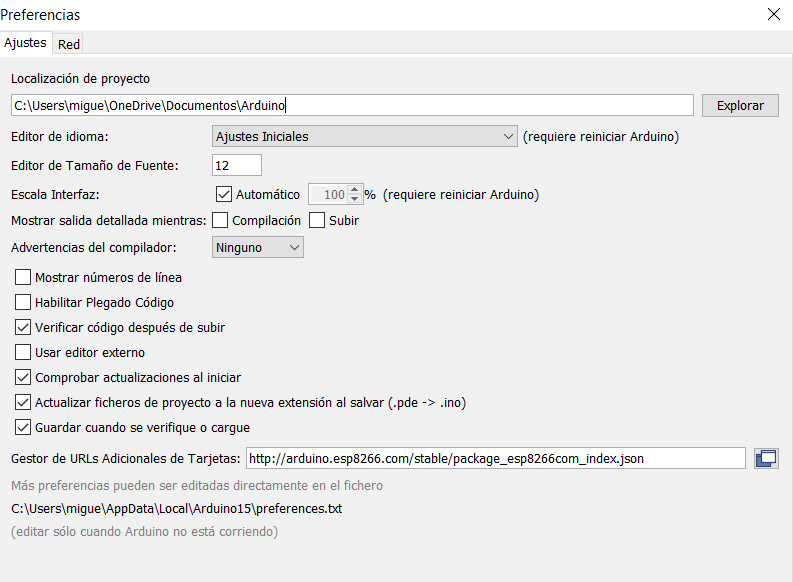
\includegraphics[scale=0.6]{imagenes/preferenciasarduino.png}
		\caption{Archivo/Preferencias}
		\label{fig:preferenciasarduino}
	\end{figure}
	
	Una vez agregada la URL accedemos a Herramientas/Placa/Gestor de tarjetas y buscamos e instalamos esp8266 by ESP8266 community (\ref{fig:instalarESP8266}).
	
	\begin{figure}[H]
		\centering
		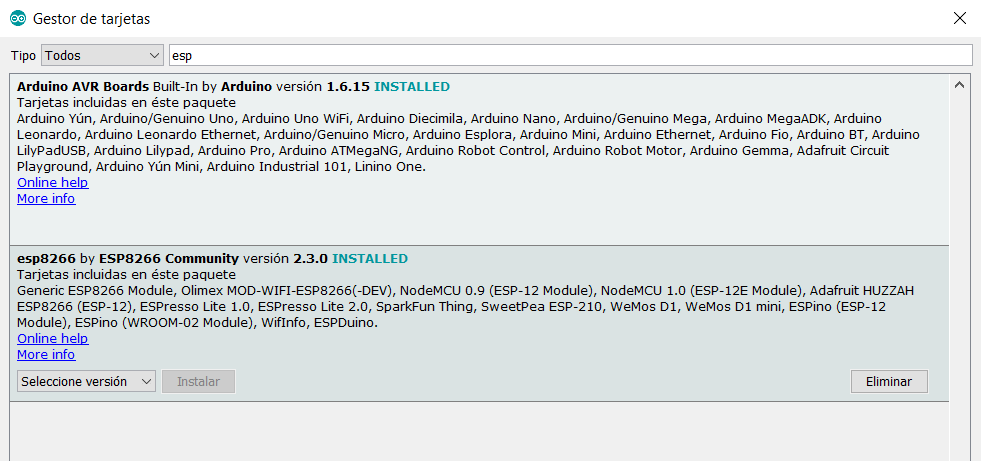
\includegraphics[scale=0.6]{imagenes/instalarESP.png}
		\caption{Herramientas/Placa/Gestor de tarjetas}
		\label{fig:instalarESP8266}
	\end{figure}
	
	En este momento tan solo nos faltará abrir el archivo .ino descargado previamente de github el cuál contiene el firmware actualizando el servidor donde queremos que se manden los datos recogidos por el sensor y las credenciales de nuestra red Wifi para que la placa ESP8266 tenga acceso a la red y pulsar sobre el botón subir para flashear el firmware a la placa.


%
%\input{capitulos/08_Conclusiones}
%
%%\chapter{Conclusiones_y_Trabajos Futuros}
%
%
%%\nocite{*}
\bibliography{bibliografia/bibliografia}\addcontentsline{toc}{chapter}{Bibliografía}
\bibliographystyle{plain}
%
%\appendix
%\input{apendices/manual_usuario/manual_usuario}
%%\input{apendices/paper/paper}
%\input{glosario/entradas_glosario}
% \addcontentsline{toc}{chapter}{Glosario}
% \printglossary
\chapter*{}
\thispagestyle{empty}

\end{document}
